\documentclass[12pt,a4paper]{ctexart}
\usepackage[top=2.5cm,bottom=2.5cm,left=2.5cm,right=2.5cm]{geometry}
\usepackage{amsmath,amssymb,amsfonts}
\usepackage{graphicx}
\usepackage{tikz}
\usetikzlibrary{shapes,arrows,positioning,calc,decorations.markings}
\usepackage{xcolor}
\usepackage{enumitem}
\usepackage{booktabs}
\usepackage{hyperref}
\usepackage{physics}
\usepackage{float}
\usepackage{caption}
\usepackage{framed}
\usepackage{tcolorbox}
\tcbuselibrary{skins,breakable}

\hypersetup{
    colorlinks=true,
    linkcolor=blue!70!black,
    citecolor=green!50!black,
    urlcolor=blue!70!black
}

% 定义颜色
\definecolor{tensorblue}{RGB}{70,130,180}
\definecolor{tensorred}{RGB}{205,92,92}
\definecolor{tensorgreen}{RGB}{60,179,113}
\definecolor{tensororange}{RGB}{230,160,50}
\definecolor{tensorpurple}{RGB}{147,112,219}
\definecolor{bgblue}{RGB}{235,245,255}

% 定义tcolorbox样式
\newtcolorbox{examplebox}[1][]{
    colback=bgblue,
    colframe=tensorblue,
    fonttitle=\bfseries,
    title={#1},
    breakable,
    enhanced
}

\newtcolorbox{keybox}[1][]{
    colback=yellow!5!white,
    colframe=tensororange,
    fonttitle=\bfseries,
    title={#1},
    breakable,
    enhanced
}

% TikZ 样式
\tikzset{
    tensor/.style={circle, draw=tensorblue, fill=tensorblue!20, thick, minimum size=1cm, font=\large},
    tensorR/.style={circle, draw=tensorred, fill=tensorred!20, thick, minimum size=1cm, font=\large},
    tensorG/.style={circle, draw=tensorgreen, fill=tensorgreen!20, thick, minimum size=1cm, font=\large},
    tensorP/.style={circle, draw=tensorpurple, fill=tensorpurple!20, thick, minimum size=1cm, font=\large},
    tensorO/.style={circle, draw=tensororange, fill=tensororange!20, thick, minimum size=1cm, font=\large},
    tensorS/.style={rectangle, draw=tensorblue, fill=tensorblue!20, thick, minimum size=0.8cm, font=\large},
    leg/.style={thick, black},
    cleg/.style={very thick, red!70!black},
    indexlabel/.style={font=\small, midway},
}

\title{\Huge\bfseries 张量网络与张量收缩\\[0.5em]
\Large 从零开始的系统介绍}
\author{自动生成}
\date{2026年3月}

\begin{document}

\maketitle
\thispagestyle{empty}

\vfill
\begin{abstract}
本文从最基础的概念出发，系统地介绍张量、张量网络与张量收缩方法。内容涵盖：张量的基本定义与图形表示法、张量收缩的数学原理与计算方法、常见的张量网络结构（MPS、MPO、PEPS、树张量网络等），以及张量网络在量子物理中的应用。文中配有大量简单易懂的例子和图示，力求让初学者能够从零建立起对张量网络的直觉理解。
\end{abstract}
\vfill

\newpage
\tableofcontents
\newpage

%=============================================================
\section{引言：为什么需要张量网络？}
%=============================================================

在量子多体物理中，我们面临一个根本性的困难：\textbf{指数墙（exponential wall）}。

考虑一个由 $N$ 个量子比特（spin-1/2 粒子）组成的系统，其一般量子态可以写为：
\begin{equation}
    \ket{\Psi} = \sum_{s_1, s_2, \ldots, s_N = 0}^{1} C_{s_1 s_2 \cdots s_N} \ket{s_1 s_2 \cdots s_N}
\end{equation}
其中系数张量 $C_{s_1 s_2 \cdots s_N}$ 有 $2^N$ 个独立分量。当 $N=40$ 时，这就需要存储约 $10^{12}$ 个复数，已经超出了普通计算机的内存；当 $N=100$ 时，$2^{100} \approx 10^{30}$，这已经远超全人类的存储能力。

\begin{keybox}[核心问题]
量子多体系统的状态空间随粒子数\textbf{指数增长}，直接存储和处理这些数据是不可能的。张量网络提供了一种\textbf{高效的参数化方案}，用远少于指数多的参数来近似描述量子态。
\end{keybox}

张量网络的核心思想很简单：把一个巨大的高阶张量，\textbf{分解}为多个小张量的\textbf{网络}，这些小张量通过\textbf{收缩}（contraction）连接在一起。这类似于：
\begin{itemize}
    \item 把一个巨大的矩阵分解为两个较小矩阵的乘积（SVD分解）
    \item 把一个复杂的函数分解为简单函数的组合
\end{itemize}

在本文中，我们将从最基础的"什么是张量"讲起，一步步建立起对张量网络的理解。

%=============================================================
\section{张量基础}
%=============================================================

\subsection{从标量到张量：逐步推广}

张量是标量、向量、矩阵的自然推广。我们用一个表格来展示这种层次关系：

\begin{table}[H]
\centering
\begin{tabular}{cccc}
\toprule
\textbf{名称} & \textbf{阶数（rank）} & \textbf{指标数} & \textbf{例子} \\
\midrule
标量（scalar） & 0 & 0 & $a = 3.14$ \\
向量（vector） & 1 & 1 & $v_i$，如 $(1, 2, 3)$ \\
矩阵（matrix） & 2 & 2 & $M_{ij}$，如 $\begin{pmatrix} 1 & 2 \\ 3 & 4 \end{pmatrix}$ \\
三阶张量 & 3 & 3 & $T_{ijk}$ \\
$n$ 阶张量 & $n$ & $n$ & $T_{i_1 i_2 \cdots i_n}$ \\
\bottomrule
\end{tabular}
\caption{从标量到高阶张量的推广}
\end{table}

\begin{examplebox}[例1：理解张量的阶]
\textbf{标量}：温度 $T = 300\,\text{K}$，只是一个数，不需要指标。

\textbf{向量}：速度 $\vec{v}$，需要一个指标 $i$ 来指定分量 $v_i$。在三维空间中，$i \in \{1,2,3\}$（对应 $x,y,z$ 方向），共3个分量。

\textbf{矩阵}：应力张量 $\sigma_{ij}$，需要两个指标。在三维空间中，$i,j \in \{1,2,3\}$，共 $3\times 3 = 9$ 个分量。

\textbf{三阶张量}：压电张量 $d_{ijk}$，需要三个指标，共 $3^3 = 27$ 个分量。可以想象为一个"三维数组"（一个立方体的数据）。

\textbf{四阶张量}：弹性模量张量 $C_{ijkl}$，需要四个指标，共 $3^4 = 81$ 个分量。
\end{examplebox}

\subsection{张量的分量表示}

一个 $n$ 阶张量 $T$ 具有 $n$ 个指标 $i_1, i_2, \ldots, i_n$，每个指标有一定的取值范围（称为该指标的\textbf{维度}或\textbf{键维度}，bond dimension）。张量的一个\textbf{分量}就是给定所有指标具体取值后对应的数：
\begin{equation}
    T_{i_1 i_2 \cdots i_n}, \quad i_k = 1, 2, \ldots, d_k
\end{equation}
其中 $d_k$ 是第 $k$ 个指标的维度。该张量总共有 $d_1 \times d_2 \times \cdots \times d_n$ 个分量。

\begin{examplebox}[例2：一个具体的三阶张量]
考虑一个三阶张量 $T_{ijk}$，其中 $i \in \{1,2\}$，$j \in \{1,2\}$，$k \in \{1,2,3\}$。

这个张量共有 $2 \times 2 \times 3 = 12$ 个分量。我们可以把它想象为两个 $2\times 3$ 的"切片"：

当 $i=1$ 时：
$\begin{pmatrix} T_{111} & T_{112} & T_{113} \\ T_{121} & T_{122} & T_{123} \end{pmatrix}
= \begin{pmatrix} 1 & 0 & 2 \\ 3 & 1 & -1 \end{pmatrix}$

当 $i=2$ 时：
$\begin{pmatrix} T_{211} & T_{212} & T_{213} \\ T_{221} & T_{222} & T_{223} \end{pmatrix}
= \begin{pmatrix} 0 & 2 & 1 \\ -1 & 4 & 0 \end{pmatrix}$
\end{examplebox}

\subsection{张量的图形表示法（Penrose图形记号）}

张量网络最强大的工具之一是其\textbf{图形表示法}（diagrammatic notation），也叫 Penrose 图形记号。规则非常简单：

\begin{keybox}[图形表示法的基本规则]
\begin{enumerate}
    \item \textbf{张量} $\longrightarrow$ 用一个\textbf{节点}（圆或方块等形状）表示
    \item \textbf{指标} $\longrightarrow$ 从节点伸出的\textbf{线}（leg，也叫"腿"）
    \item $n$ 阶张量有 $n$ 条腿
    \item \textbf{收缩}（求和）$\longrightarrow$ 两条腿\textbf{相连}
\end{enumerate}
\end{keybox}

\begin{figure}[H]
\centering
\begin{tikzpicture}[scale=1]
    % 标量
    \node[tensor] (s) at (0,0) {$a$};
    \node[below=0.5cm] at (s) {标量（0阶）};

    % 向量
    \node[tensor] (v) at (3,0) {$v$};
    \draw[leg] (v) -- ++(1.2,0) node[right] {$i$};
    \node[below=0.5cm] at (v) {向量（1阶）};

    % 矩阵
    \node[tensor] (m) at (7,0) {$M$};
    \draw[leg] (m) -- ++(-1.2,0) node[left] {$i$};
    \draw[leg] (m) -- ++(1.2,0) node[right] {$j$};
    \node[below=0.5cm] at (m) {矩阵（2阶）};

    % 三阶张量
    \node[tensor] (t) at (11,0) {$T$};
    \draw[leg] (t) -- ++(-1.2,0) node[left] {$i$};
    \draw[leg] (t) -- ++(1.2,0) node[right] {$k$};
    \draw[leg] (t) -- ++(0,1.2) node[above] {$j$};
    \node[below=0.5cm] at (t) {三阶张量};
\end{tikzpicture}
\caption{不同阶张量的图形表示}
\end{figure}

\begin{examplebox}[例3：用图形理解张量的形状]
量子力学中的密度矩阵 $\rho_{ij}$ 是一个二阶张量（矩阵），用一个带两条腿的节点表示。

一个量子门（如CNOT门）作用在两个量子比特上，可以表示为四阶张量 $U_{i_1 i_2 j_1 j_2}$，其中 $i_1, i_2$ 是输入指标，$j_1, j_2$ 是输出指标——画出来就是一个带四条腿的节点。
\end{examplebox}

%=============================================================
\section{张量收缩}
%=============================================================

\subsection{什么是张量收缩？}

张量收缩是张量运算中最核心的操作。直观地说，就是对两个张量的\textbf{共同指标求和}。

\begin{keybox}[张量收缩的定义]
给定两个张量 $A$ 和 $B$，如果它们共享一个或多个指标，对这些共同指标求和就得到一个新的张量。这个过程叫做\textbf{张量收缩}（tensor contraction）。
\end{keybox}

用数学语言表达：如果 $A_{ijk}$ 和 $B_{klm}$ 共享指标 $k$，则收缩后得到：
\begin{equation}
    C_{ijlm} = \sum_{k} A_{ijk} \, B_{klm}
\end{equation}

在图形表示法中，收缩就是把两个张量对应的腿\textbf{连起来}：

\begin{figure}[H]
\centering
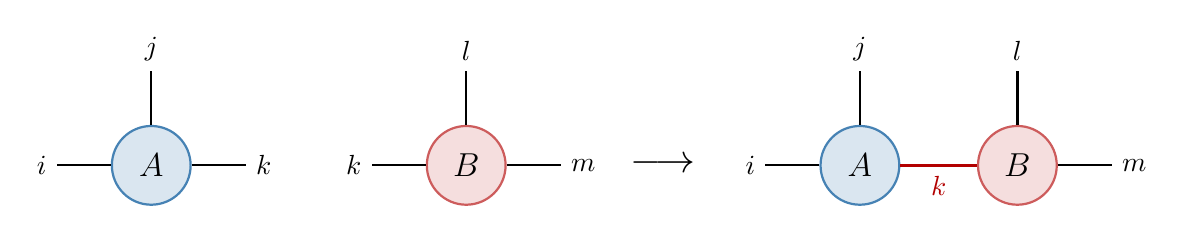
\begin{tikzpicture}[scale=1]
    % Before contraction
    \node[tensor] (A) at (0,0) {$A$};
    \draw[leg] (A) -- ++(-1.2,0) node[left] {$i$};
    \draw[leg] (A) -- ++(0,1.2) node[above] {$j$};
    \draw[leg] (A) -- ++(1.2,0) node[right] {$k$};

    \node[tensorR] (B) at (4,0) {$B$};
    \draw[leg] (B) -- ++(-1.2,0) node[left] {$k$};
    \draw[leg] (B) -- ++(1.2,0) node[right] {$m$};
    \draw[leg] (B) -- ++(0,1.2) node[above] {$l$};

    \node at (6.5,0) {\Large $\longrightarrow$};

    % After contraction
    \node[tensor] (A2) at (9,0) {$A$};
    \draw[leg] (A2) -- ++(-1.2,0) node[left] {$i$};
    \draw[leg] (A2) -- ++(0,1.2) node[above] {$j$};

    \node[tensorR] (B2) at (11,0) {$B$};
    \draw[leg] (B2) -- ++(1.2,0) node[right] {$m$};
    \draw[leg] (B2) -- ++(0,1.2) node[above] {$l$};

    \draw[cleg] (A2) -- (B2) node[midway, below] {$k$};
\end{tikzpicture}
\caption{张量收缩的图形表示：共享指标 $k$ 的两条腿连在一起}
\end{figure}

\subsection{熟悉的操作都是张量收缩}

你已经熟知的许多线性代数操作，其实都是张量收缩的特殊情况！

\subsubsection{（1）向量内积}

两个向量 $u_i$ 和 $v_i$ 的内积：
\begin{equation}
    \vec{u} \cdot \vec{v} = \sum_i u_i \, v_i = \text{一个标量}
\end{equation}

\begin{figure}[H]
\centering
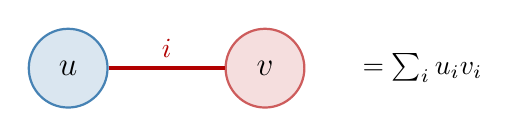
\begin{tikzpicture}
    \node[tensor] (u) at (0,0) {$u$};
    \node[tensorR] (v) at (2.5,0) {$v$};
    \draw[cleg] (u) -- (v) node[midway, above] {$i$};
    \node at (4.5,0) {$= \sum_i u_i v_i$};
\end{tikzpicture}
\caption{向量内积：两个一阶张量收缩，结果是零阶张量（标量）}
\end{figure}

\begin{examplebox}[例4：向量内积的张量收缩]
设 $u = (1, 2, 3)$，$v = (4, 5, 6)$，则：
\[
\sum_i u_i v_i = 1\times 4 + 2\times 5 + 3\times 6 = 4 + 10 + 18 = 32
\]
两个1阶张量（各1条腿），收缩后得到0阶张量（标量，0条腿）。
\end{examplebox}

\subsubsection{（2）矩阵-向量乘法}

矩阵 $M_{ij}$ 作用在向量 $v_j$ 上：
\begin{equation}
    w_i = \sum_j M_{ij} \, v_j
\end{equation}

\begin{figure}[H]
\centering
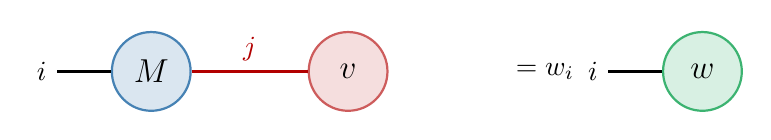
\begin{tikzpicture}
    \node[tensor] (M) at (0,0) {$M$};
    \draw[leg] (M) -- ++(-1.2,0) node[left] {$i$};
    \node[tensorR] (v) at (2.5,0) {$v$};
    \draw[cleg] (M) -- (v) node[midway, above] {$j$};
    \node at (5,0) {$= w_i$};
    \node[tensorG] (w) at (7,0) {$w$};
    \draw[leg] (w) -- ++(-1.2,0) node[left] {$i$};
\end{tikzpicture}
\caption{矩阵-向量乘法：2阶张量与1阶张量收缩，得到1阶张量}
\end{figure}

\begin{examplebox}[例5：矩阵-向量乘法]
\[
\begin{pmatrix} 1 & 2 \\ 3 & 4 \end{pmatrix} \begin{pmatrix} 5 \\ 6 \end{pmatrix}
= \begin{pmatrix} 1\times5 + 2\times6 \\ 3\times5 + 4\times6 \end{pmatrix}
= \begin{pmatrix} 17 \\ 39 \end{pmatrix}
\]
这里对指标 $j$ 求和（$j=1,2$），留下指标 $i$。
\end{examplebox}

\subsubsection{（3）矩阵乘法}

两个矩阵 $A_{ik}$ 和 $B_{kj}$ 的乘法：
\begin{equation}
    C_{ij} = \sum_k A_{ik} \, B_{kj}
\end{equation}

\begin{figure}[H]
\centering
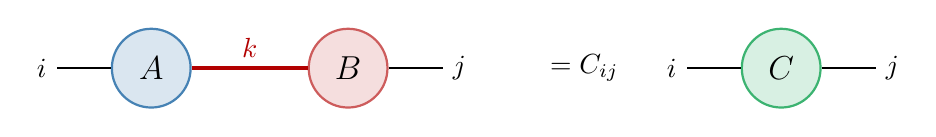
\begin{tikzpicture}
    \node[tensor] (A) at (0,0) {$A$};
    \draw[leg] (A) -- ++(-1.2,0) node[left] {$i$};
    \node[tensorR] (B) at (2.5,0) {$B$};
    \draw[cleg] (A) -- (B) node[midway, above] {$k$};
    \draw[leg] (B) -- ++(1.2,0) node[right] {$j$};
    \node at (5.5,0) {$= C_{ij}$};
    \node[tensorG] (C) at (8,0) {$C$};
    \draw[leg] (C) -- ++(-1.2,0) node[left] {$i$};
    \draw[leg] (C) -- ++(1.2,0) node[right] {$j$};
\end{tikzpicture}
\caption{矩阵乘法：两个2阶张量收缩一个指标，得到2阶张量}
\end{figure}

\subsubsection{（4）矩阵的迹}

矩阵 $A_{ij}$ 的迹是对\textbf{同一个张量}的两个指标做收缩：
\begin{equation}
    \text{tr}(A) = \sum_i A_{ii}
\end{equation}

\begin{figure}[H]
\centering
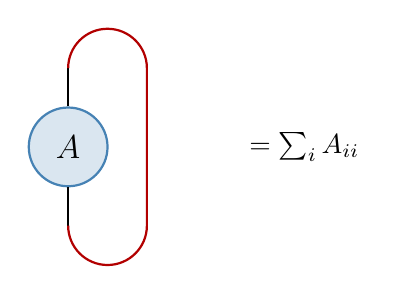
\begin{tikzpicture}
    \node[tensor] (A) at (0,0) {$A$};
    \draw[leg] (A) -- ++(0,1);
    \draw[leg] (A) -- ++(0,-1);
    \draw[thick, red!70!black] (0,1) arc (180:0:0.5) -- ++(0,-2) arc (0:-180:0.5);
    \node at (3,0) {$= \sum_i A_{ii}$};
\end{tikzpicture}
\caption{矩阵的迹：同一个张量的两条腿连起来}
\end{figure}

\begin{examplebox}[例6：矩阵的迹]
\[
\text{tr}\begin{pmatrix} 1 & 2 \\ 3 & 4 \end{pmatrix} = A_{11} + A_{22} = 1 + 4 = 5
\]
\end{examplebox}

\subsubsection{（5）外积（张量积）}

两个向量 $u_i$ 和 $v_j$ 的外积\textbf{不收缩}任何指标：
\begin{equation}
    T_{ij} = u_i \, v_j
\end{equation}

\begin{figure}[H]
\centering
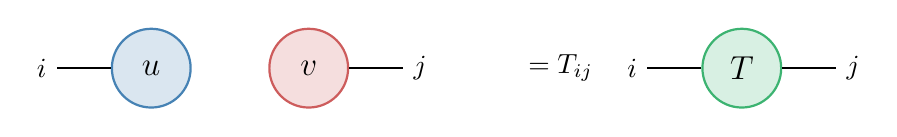
\begin{tikzpicture}
    \node[tensor] (u) at (0,0) {$u$};
    \draw[leg] (u) -- ++(-1.2,0) node[left] {$i$};
    \node[tensorR] (v) at (2,0) {$v$};
    \draw[leg] (v) -- ++(1.2,0) node[right] {$j$};
    \node at (5.2,0) {$= T_{ij}$};
    \node[tensorG] (T) at (7.5,0) {$T$};
    \draw[leg] (T) -- ++(-1.2,0) node[left] {$i$};
    \draw[leg] (T) -- ++(1.2,0) node[right] {$j$};
\end{tikzpicture}
\caption{外积：两个张量放在一起但不连接任何腿}
\end{figure}

\begin{examplebox}[例7：外积]
\[
u = \begin{pmatrix} 1 \\ 2 \end{pmatrix}, \quad v = \begin{pmatrix} 3 \\ 4 \\ 5 \end{pmatrix}
\quad \Rightarrow \quad
T_{ij} = u_i v_j = \begin{pmatrix} 3 & 4 & 5 \\ 6 & 8 & 10 \end{pmatrix}
\]
\end{examplebox}

\subsection{张量收缩的计算复杂度}

理解收缩的计算代价非常重要。对于两个张量的收缩 $C_{ijlm} = \sum_k A_{ijk} B_{klm}$，假设所有指标维度都是 $d$，则：
\begin{itemize}
    \item 结果张量 $C$ 有 $d^4$ 个元素
    \item 每个元素需要对 $k$ 求和，做 $d$ 次乘加运算
    \item 总计算量：$O(d^5)$
\end{itemize}

\begin{keybox}[收缩的一般复杂度]
收缩两个张量时，计算复杂度为：
\[
    O\left(\prod_{\text{所有指标}} d_k\right)
\]
即所有涉及的指标（包括被收缩的和保留的）的维度之积。
\end{keybox}

\begin{examplebox}[例8：矩阵乘法的复杂度]
矩阵乘法 $C_{ij} = \sum_k A_{ik} B_{kj}$，三个指标 $i,j,k$ 各取 $d$ 个值。

计算量：$O(d^3)$。这就是我们熟知的矩阵乘法 $O(n^3)$ 复杂度。
\end{examplebox}

%=============================================================
\section{张量网络的基本概念}
%=============================================================

\subsection{什么是张量网络？}

\begin{keybox}[张量网络的定义]
\textbf{张量网络}（Tensor Network）是由多个张量通过指标收缩连接而成的网络结构。在图形表示中，它表现为多个节点通过线相连的图。
\end{keybox}

更具体地说，一个张量网络定义了一种将高阶张量\textbf{分解}为多个低阶张量的方式。通过控制低阶张量的大小（即\textbf{键维度}，bond dimension $D$），我们可以用远少于指数多的参数来近似表示一个高阶张量。

\begin{figure}[H]
\centering
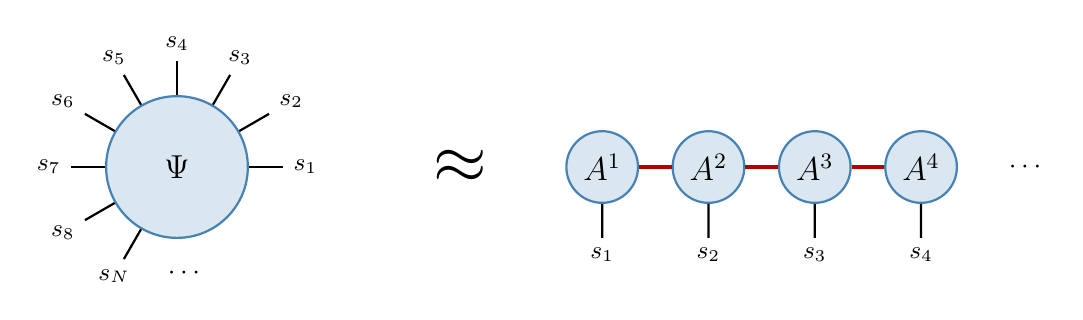
\begin{tikzpicture}[scale=0.9]
    % Big tensor
    \node[tensor, minimum size=1.8cm] (big) at (0,0) {$\Psi$};
    \foreach \angle/\label in {0/1, 30/2, 60/3, 90/4, 120/5, 150/6, 180/7, 210/8, 240/N} {
        \draw[leg] (big) -- ++(\angle:1.5) node[anchor=\angle+180, font=\small] {$s_{\label}$};
    }
    \node at (275:1.5) {$\cdots$};

    \node at (4, 0) {\Huge $\approx$};

    % Tensor network (MPS)
    \foreach \x/\label in {6/1, 7.5/2, 9/3, 10.5/4} {
        \node[tensor, minimum size=0.7cm] (t\label) at (\x, 0) {$A^{\label}$};
        \draw[leg] (t\label) -- ++(0,-1) node[below, font=\small] {$s_{\label}$};
    }
    \draw[cleg] (t1) -- (t2);
    \draw[cleg] (t2) -- (t3);
    \draw[cleg] (t3) -- (t4);
    \node at (12, 0) {$\cdots$};
\end{tikzpicture}
\caption{张量网络的核心思想：用一组小张量的网络来近似一个巨大的高阶张量}
\end{figure}

\subsection{开放指标与内部指标}

在张量网络中，有两类指标：

\begin{itemize}
    \item \textbf{开放指标}（open/physical indices）：没有被收缩的指标，对应图中\textbf{悬空的腿}。这些通常是\textbf{物理指标}，例如每个格点的自旋状态。
    \item \textbf{内部指标}（internal/bond indices）：被收缩的指标，对应图中\textbf{连接两个节点的线}。这些是\textbf{辅助指标}，其维度 $D$ 称为\textbf{键维度}（bond dimension），控制张量网络的表达能力。
\end{itemize}

\begin{figure}[H]
\centering
\begin{tikzpicture}
    \node[tensor] (A) at (0,0) {$A$};
    \node[tensorR] (B) at (3,0) {$B$};
    \node[tensorG] (C) at (6,0) {$C$};

    % Physical legs (open)
    \draw[leg] (A) -- ++(0,-1.2) node[below] {$s_1$};
    \draw[leg] (B) -- ++(0,-1.2) node[below] {$s_2$};
    \draw[leg] (C) -- ++(0,-1.2) node[below] {$s_3$};

    % Bond legs (internal)
    \draw[cleg] (A) -- (B) node[midway, above] {$\alpha_1$};
    \draw[cleg] (B) -- (C) node[midway, above] {$\alpha_2$};

    % Labels
    \draw[<-, gray, thick] (0,-1.5) -- ++(0,-0.8) node[below, font=\small, black] {物理指标 $d$维};
    \draw[<-, gray, thick] (1.5,0.5) -- ++(0,0.8) node[above, font=\small, black] {键指标 $D$维};
\end{tikzpicture}
\caption{物理指标（向下的腿）与键指标（水平连接线）}
\end{figure}

\subsection{参数量的巨大节省}

这就是张量网络的威力所在。以 $N$ 个自旋-1/2 粒子为例：

\begin{table}[H]
\centering
\begin{tabular}{lcc}
\toprule
\textbf{表示方式} & \textbf{参数数量} & $N=100$时 \\
\midrule
完整张量 $C_{s_1\cdots s_N}$ & $2^N$ & $\sim 10^{30}$ \\
张量网络（键维度$D$） & $N \times d \times D^2$ & $\sim 100 \times 2 \times D^2$ \\
MPS, $D=100$ & --- & $2 \times 10^6$ \\
\bottomrule
\end{tabular}
\caption{参数量对比：指数 vs 多项式}
\end{table}

从 $10^{30}$ 个参数压缩到 $10^6$ 个，这就是张量网络的力量！

当然，代价是张量网络并不能精确表示所有量子态——它只能表示一类"低纠缠"的态。幸运的是，物理中许多重要的态（如基态）恰好就属于这一类。

%=============================================================
\section{常见的张量网络结构}
%=============================================================

\subsection{矩阵乘积态（MPS）}

\textbf{矩阵乘积态}（Matrix Product State，MPS）是最基本、也是目前应用最广泛的张量网络结构。它的核心思想是：\textbf{把一个描述整体量子态的巨大高阶张量，拆解成一条链上每个格点各一个小张量，然后通过矩阵乘法把它们串联起来}。

\paragraph{回顾问题：} 在第1节中我们看到，一个 $N$ 体量子态的系数张量 $C_{s_1 s_2 \cdots s_N}$ 有 $d^N$ 个分量（$d$ 是每个格点的物理自由度数，比如自旋-$1/2$ 时 $d=2$）。这个张量太大了，无法直接存储。MPS 提供了一种巧妙的近似方案。

\paragraph{MPS的基本公式：} MPS 将系数张量写成如下形式：

\begin{equation}
    C_{s_1 s_2 \cdots s_N} = \sum_{\alpha_1, \alpha_2, \ldots} A^{s_1}_{\alpha_0 \alpha_1} A^{s_2}_{\alpha_1 \alpha_2} \cdots A^{s_N}_{\alpha_{N-1} \alpha_N}
\end{equation}

这个公式初看可能令人困惑，下面我们逐步拆解它的含义。

\paragraph{每个格点对应一个小张量：} 对于链上的第 $n$ 个格点，我们引入一个三阶张量 $A^{s_n}_{\alpha_{n-1}\alpha_n}$，它有三个指标：
\begin{itemize}
    \item \textbf{物理指标} $s_n$：描述该格点的物理状态。例如对自旋-$1/2$ 系统，$s_n$ 取值为 $\uparrow$ 或 $\downarrow$（即 $0$ 或 $1$），所以 $s_n$ 的维度 $d=2$。
    \item \textbf{左键指标} $\alpha_{n-1}$：连接到左边相邻张量的辅助指标，维度为 $D$。
    \item \textbf{右键指标} $\alpha_n$：连接到右边相邻张量的辅助指标，维度也为 $D$。
\end{itemize}
这里 $D$ 被称为\textbf{键维度}（bond dimension），它是 MPS 中最重要的参数——$D$ 越大，MPS 能表示的量子态范围就越广，但计算代价也越高。

\paragraph{为什么叫"矩阵乘积"？} 关键在于：当我们固定物理指标 $s_n$ 的取值后，剩下的两个键指标 $\alpha_{n-1}$ 和 $\alpha_n$ 恰好构成一个 $D \times D$ 的矩阵。换句话说：
\begin{itemize}
    \item 当 $s_n = 0$ 时，$A^{s_n=0}$ 是一个 $D \times D$ 矩阵；
    \item 当 $s_n = 1$ 时，$A^{s_n=1}$ 是另一个 $D \times D$ 矩阵。
\end{itemize}
所以，\textbf{每个格点实际上存储了 $d$ 个矩阵}（有多少种物理状态就有多少个矩阵）。要计算某个特定自旋构型 $(s_1, s_2, \ldots, s_N)$ 对应的系数 $C_{s_1 s_2 \cdots s_N}$，只需要：
\begin{enumerate}
    \item 根据每个格点的自旋值 $s_n$，从该格点的 $d$ 个矩阵中选出对应的那个矩阵 $A^{s_n}$；
    \item 将选出的 $N$ 个矩阵按顺序相乘：$A^{s_1} \cdot A^{s_2} \cdots A^{s_N}$；
    \item 乘积的结果（对于开放边界条件，首尾张量退化为行向量和列向量，最终得到一个标量）就是系数 $C_{s_1 s_2 \cdots s_N}$。
\end{enumerate}
这就是"矩阵乘积态"名称的由来——\textbf{量子态的每个系数都是一串矩阵乘积的结果}。

\paragraph{直观类比：} 可以把 MPS 想象成一条流水线。每个格点是流水线上的一个工位，信息（键指标）从左到右逐站传递。每个工位根据自己的物理状态（$s_n$）选择一个"加工方式"（矩阵 $A^{s_n}$），对传递过来的信息做一次线性变换。最终，经过所有工位加工后的结果就是该自旋构型的量子振幅。

\begin{figure}[H]
\centering
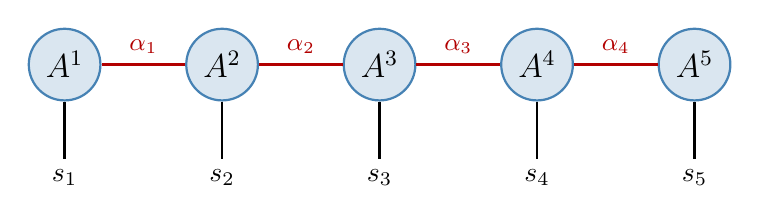
\begin{tikzpicture}[scale=1]
    \foreach \x/\label in {0/1, 2/2, 4/3, 6/4, 8/5} {
        \node[tensor, minimum size=0.8cm] (A\label) at (\x, 0) {$A^{\label}$};
        \draw[leg] (A\label) -- ++(0,-1.2) node[below] {$s_{\label}$};
    }
    \draw[cleg] (A1) -- (A2) node[midway, above, font=\small] {$\alpha_1$};
    \draw[cleg] (A2) -- (A3) node[midway, above, font=\small] {$\alpha_2$};
    \draw[cleg] (A3) -- (A4) node[midway, above, font=\small] {$\alpha_3$};
    \draw[cleg] (A4) -- (A5) node[midway, above, font=\small] {$\alpha_4$};
\end{tikzpicture}
\caption{矩阵乘积态（MPS）的图形表示}
\end{figure}

\begin{examplebox}[例9：最简单的MPS——两个量子比特]
考虑两个量子比特的 Bell 态：
\[
\ket{\Psi} = \frac{1}{\sqrt{2}}\left(\ket{00} + \ket{11}\right)
\]
系数为：$C_{00} = C_{11} = \frac{1}{\sqrt{2}}$，$C_{01} = C_{10} = 0$。

我们可以用 MPS 表示：$C_{s_1 s_2} = \sum_\alpha A^{s_1}_\alpha B^{s_2}_\alpha$。

取键维度 $D=2$，令：
\[
A^{0} = \begin{pmatrix} \frac{1}{\sqrt[4]{2}} & 0 \end{pmatrix}, \quad
A^{1} = \begin{pmatrix} 0 & \frac{1}{\sqrt[4]{2}} \end{pmatrix}
\]
\[
B^{0} = \begin{pmatrix} \frac{1}{\sqrt[4]{2}} \\ 0 \end{pmatrix}, \quad
B^{1} = \begin{pmatrix} 0 \\ \frac{1}{\sqrt[4]{2}} \end{pmatrix}
\]

验证：
\begin{align}
C_{00} &= A^0 B^0 = \frac{1}{\sqrt[4]{2}} \cdot \frac{1}{\sqrt[4]{2}} = \frac{1}{\sqrt{2}} \quad \checkmark \\
C_{01} &= A^0 B^1 = \frac{1}{\sqrt[4]{2}} \cdot 0 + 0 \cdot \frac{1}{\sqrt[4]{2}} = 0 \quad \checkmark \\
C_{10} &= A^1 B^0 = 0 \cdot \frac{1}{\sqrt[4]{2}} + \frac{1}{\sqrt[4]{2}} \cdot 0 = 0 \quad \checkmark \\
C_{11} &= A^1 B^1 = 0 \cdot 0 + \frac{1}{\sqrt[4]{2}} \cdot \frac{1}{\sqrt[4]{2}} = \frac{1}{\sqrt{2}} \quad \checkmark
\end{align}
\end{examplebox}

\begin{examplebox}[例10：GHZ态的MPS表示]
三量子比特 GHZ 态 $\ket{\text{GHZ}} = \frac{1}{\sqrt{2}}(\ket{000} + \ket{111})$ 可以用键维度 $D=2$ 的 MPS 表示：
\[
A^{0} = \begin{pmatrix} 1 & 0 \end{pmatrix}, \quad A^{1} = \begin{pmatrix} 0 & 1 \end{pmatrix}
\]
\[
B^{0} = \begin{pmatrix} 1 & 0 \\ 0 & 0 \end{pmatrix}, \quad B^{1} = \begin{pmatrix} 0 & 0 \\ 0 & 1 \end{pmatrix}
\]
\[
C^{0} = \begin{pmatrix} \frac{1}{\sqrt{2}} \\ 0 \end{pmatrix}, \quad C^{1} = \begin{pmatrix} 0 \\ \frac{1}{\sqrt{2}} \end{pmatrix}
\]
读者可以验证：$A^{s_1} B^{s_2} C^{s_3}$ 仅当 $s_1 = s_2 = s_3$ 时非零。
\end{examplebox}

\subsubsection*{详细应用实例：用转移矩阵法求解一维 Ising 模型}

前面的例子展示了如何用 MPS 表示简单的量子态。现在，我们用一个真正重要的物理问题来展示张量网络的威力：\textbf{二维 Ising 模型}。

二维 Ising 模型是统计力学中最经典的模型之一——它是第一个被严格证明存在相变的模型（Onsager, 1944）。我们将从头到尾展示：如何把二维 Ising 模型的配分函数表示为一个二维张量网络，然后用\textbf{角转移矩阵}（Corner Transfer Matrix, CTM）方法来收缩这个网络，从而精确计算自由能、磁化强度、比热等热力学量。

这个例子将展示张量网络方法在处理二维问题时的核心思路——与一维的转移矩阵法（$Z = \mathrm{Tr}(\mathbf{T}^N)$）不同，二维问题需要更精巧的收缩策略。

\paragraph{（1）模型定义}

一维 Ising 模型描述一条链上 $N$ 个自旋的相互作用。每个格点 $i$ 上有一个自旋变量 $\sigma_i$，只能取 $+1$（向上）或 $-1$（向下）两个值。系统的哈密顿量为：
\begin{equation}
    H = -J \sum_{i=1}^{N} \sigma_i \sigma_{i+1} - h \sum_{i=1}^{N} \sigma_i
\end{equation}
其中：
\begin{itemize}
    \item $J > 0$：最近邻耦合常数。$J>0$ 表示铁磁相互作用（相邻自旋倾向于平行排列）。
    \item $h$：外加磁场。$h>0$ 倾向于让自旋向上。
    \item 我们采用\textbf{周期边界条件}：$\sigma_{N+1} = \sigma_1$，即链首尾相连形成环。
\end{itemize}

统计力学的核心任务是计算\textbf{配分函数}：
\begin{equation}
    Z = \sum_{\{\sigma\}} e^{-\beta H} = \sum_{\sigma_1 = \pm 1} \sum_{\sigma_2 = \pm 1} \cdots \sum_{\sigma_N = \pm 1} \exp\!\left(\beta J \sum_{i} \sigma_i \sigma_{i+1} + \beta h \sum_{i} \sigma_i\right)
\end{equation}
其中 $\beta = 1/(k_B T)$ 是逆温度。一旦知道了 $Z$，所有热力学量都可以通过对 $Z$ 求导得到。

\textbf{困难在哪里？} 直接求和需要遍历所有 $2^N$ 种自旋构型。对于 $N = 100$ 的链，就有 $2^{100} \approx 10^{30}$ 种构型——不可能逐一枚举。转移矩阵法的精妙之处在于，它把这个指数级的求和问题\textbf{归结为一个 $2 \times 2$ 矩阵的 $N$ 次方}，从而实现精确求解。

\paragraph{（2）关键思想：将 Boltzmann 权重分解为局部因子}

我们注意到，指数函数的一个重要性质是 $e^{a+b} = e^a \cdot e^b$。利用这个性质，可以把整体的 Boltzmann 权重拆成逐对相互作用的乘积。

首先，为了对称地处理磁场项，我们把 $\sigma_i$ 上的磁场能量均分到它与左邻居、右邻居的两个键上：
\begin{equation}
    h \sum_{i} \sigma_i = \sum_{i} \frac{h}{2}(\sigma_i + \sigma_{i+1})
\end{equation}
（在周期边界条件下，每个 $\sigma_i$ 恰好出现两次，所以两边相等。）

这样，Boltzmann 权重可以写成：
\begin{equation}
    e^{-\beta H} = \prod_{i=1}^{N} \exp\!\left[\beta J \sigma_i \sigma_{i+1} + \frac{\beta h}{2}(\sigma_i + \sigma_{i+1})\right]
\end{equation}

我们把每一个因子定义为\textbf{转移矩阵的矩阵元}。

\paragraph{（3）构造转移矩阵}

定义 $2 \times 2$ 的\textbf{转移矩阵} $\mathbf{T}$，其矩阵元为：
\begin{equation}
    T_{\sigma, \sigma'} = \exp\!\left[\beta J \,\sigma \sigma' + \frac{\beta h}{2}(\sigma + \sigma')\right]
\end{equation}
其中 $\sigma, \sigma' = \pm 1$ 分别标记行和列。

为了简洁，定义无量纲参数：
\[
K \equiv \beta J = \frac{J}{k_B T}, \qquad \tilde{h} \equiv \beta h = \frac{h}{k_B T}
\]
则 $T_{\sigma, \sigma'} = e^{K \sigma\sigma' + \tilde{h}(\sigma + \sigma')/2}$。

现在，我们逐个写出矩阵元。$\sigma$ 和 $\sigma'$ 各有两种取值 $+1$ 和 $-1$，所以共有四个矩阵元：
\begin{align}
T_{+1,+1} &= e^{K \cdot (+1)(+1) + \tilde{h} \cdot (+1+1)/2} = e^{K + \tilde{h}} \\
T_{+1,-1} &= e^{K \cdot (+1)(-1) + \tilde{h} \cdot (+1-1)/2} = e^{-K} \\
T_{-1,+1} &= e^{K \cdot (-1)(+1) + \tilde{h} \cdot (-1+1)/2} = e^{-K} \\
T_{-1,-1} &= e^{K \cdot (-1)(-1) + \tilde{h} \cdot (-1-1)/2} = e^{K - \tilde{h}}
\end{align}

用矩阵形式写出来（行对应 $\sigma = +1, -1$，列对应 $\sigma' = +1, -1$）：
\begin{equation}
\boxed{
\mathbf{T} = \begin{pmatrix} e^{K + \tilde{h}} & e^{-K} \\ e^{-K} & e^{K - \tilde{h}} \end{pmatrix}
}
\end{equation}

\textbf{注意：} 这个 $\mathbf{T}$ 是一个实对称矩阵（因为 $T_{+1,-1} = T_{-1,+1} = e^{-K}$），所以它一定可以对角化，且有实本征值。

\paragraph{（4）配分函数 = 矩阵乘积的迹}

现在，配分函数的求和可以重新组织。原来的求和是：
\[
Z = \sum_{\sigma_1, \sigma_2, \ldots, \sigma_N} T_{\sigma_1, \sigma_2} \cdot T_{\sigma_2, \sigma_3} \cdots T_{\sigma_N, \sigma_1}
\]

让我们仔细看这个求和的结构。先固定 $\sigma_1$，对 $\sigma_2$ 求和：
\[
\sum_{\sigma_2} T_{\sigma_1, \sigma_2} \cdot T_{\sigma_2, \sigma_3} = (\mathbf{T}^2)_{\sigma_1, \sigma_3}
\]
这正是矩阵乘法的定义！继续对 $\sigma_3, \sigma_4, \ldots$ 依次求和，最终得到 $(\mathbf{T}^N)_{\sigma_1, \sigma_1}$。最后对 $\sigma_1$ 求和，就是矩阵的\textbf{迹}（trace）：
\begin{equation}
\boxed{
Z = \mathrm{Tr}\!\left(\mathbf{T}^N\right) = \sum_{\sigma_1} (\mathbf{T}^N)_{\sigma_1, \sigma_1}
}
\end{equation}

\textbf{这就是整个转移矩阵法最核心的等式。} 我们把一个对 $2^N$ 种构型的求和，\textbf{等价地}变成了一个 $2 \times 2$ 矩阵的 $N$ 次方再取迹——计算量从指数级骤降为多项式级。

\paragraph{（5）与 MPS 的深层联系}

让我们暂停一下，仔细对比 $Z = \mathrm{Tr}(\mathbf{T}^N)$ 和 MPS 公式。MPS 的核心公式是：
\[
C_{s_1 s_2 \cdots s_N} = \sum_{\alpha_1, \alpha_2, \ldots} A^{s_1}_{\alpha_0 \alpha_1} A^{s_2}_{\alpha_1 \alpha_2} \cdots A^{s_N}_{\alpha_{N-1} \alpha_N}
\]

而配分函数可以写成：
\[
Z = \sum_{\sigma_1, \ldots, \sigma_N} \; \sum_{\text{（无额外键指标）}} T_{\sigma_1, \sigma_2} \cdot T_{\sigma_2, \sigma_3} \cdots T_{\sigma_N, \sigma_1}
\]

对比可以发现：
\begin{itemize}
    \item 在 MPS 中，$s_n$ 是物理指标（开放的），$\alpha_n$ 是键指标（被求和/收缩的）。
    \item 在转移矩阵中，$\sigma_n$ \textbf{既是物理指标又是键指标}——它既标记格点 $n$ 的自旋状态，又在求和时扮演连接相邻转移矩阵的角色。
    \item 配分函数 $Z$ 是对\textbf{所有}指标求和（包括物理指标），所以它是一个标量；而 MPS 保留物理指标，给出的是每个构型的系数。
\end{itemize}

换句话说，\textbf{转移矩阵法就是经典统计力学中的"MPS"结构}。一维 Ising 模型的配分函数天然具有矩阵乘积的形式，键维度恰好是 $D = 2$（因为每个自旋有两种取值）。

\paragraph{（6）对角化转移矩阵}

为了计算 $\mathbf{T}^N$，我们需要对角化 $\mathbf{T}$。先从\textbf{零外场}（$h = 0$，即 $\tilde{h} = 0$）的简单情况入手。

\subparagraph{零外场情况（$h = 0$）：}
此时转移矩阵简化为：
\[
\mathbf{T} = \begin{pmatrix} e^K & e^{-K} \\ e^{-K} & e^K \end{pmatrix}
\]

这是一个以 $e^K$ 为对角元、$e^{-K}$ 为非对角元的对称矩阵。求本征值 $\lambda$：
\[
\det(\mathbf{T} - \lambda \mathbf{I}) = (e^K - \lambda)^2 - e^{-2K} = 0
\]
\[
e^K - \lambda = \pm e^{-K}
\]
\begin{equation}
\boxed{
\lambda_+ = e^K + e^{-K} = 2\cosh K, \qquad \lambda_- = e^K - e^{-K} = 2\sinh K
}
\end{equation}

对应的归一化本征向量为：
\[
|+\rangle = \frac{1}{\sqrt{2}}\begin{pmatrix} 1 \\ 1 \end{pmatrix}, \qquad |-\rangle = \frac{1}{\sqrt{2}}\begin{pmatrix} 1 \\ -1 \end{pmatrix}
\]

注意 $\lambda_+ > \lambda_- > 0$（因为 $\cosh K > \sinh K > 0$ 对任意 $K > 0$），所以 $\lambda_+$ 是\textbf{最大本征值}。

\subparagraph{含外场的一般情况（$h \neq 0$）：}
对一般的转移矩阵，利用迹和行列式：
\begin{align}
\mathrm{Tr}\,\mathbf{T} &= e^{K+\tilde{h}} + e^{K-\tilde{h}} = 2e^K \cosh\tilde{h} \\
\det\mathbf{T} &= e^{K+\tilde{h}} \cdot e^{K-\tilde{h}} - e^{-2K} = e^{2K} - e^{-2K} = 2\sinh(2K)
\end{align}

由韦达定理 $\lambda_\pm = \frac{1}{2}\!\left[\mathrm{Tr}\,\mathbf{T} \pm \sqrt{(\mathrm{Tr}\,\mathbf{T})^2 - 4\det\mathbf{T}}\right]$，判别式为：
\[
(\mathrm{Tr}\,\mathbf{T})^2 - 4\det\mathbf{T} = 4e^{2K}\cosh^2\!\tilde{h} - 4(e^{2K} - e^{-2K}) = 4e^{2K}\sinh^2\!\tilde{h} + 4e^{-2K}
\]

因此：
\begin{equation}
\boxed{
\lambda_\pm = e^K \cosh\tilde{h} \pm \sqrt{e^{2K}\sinh^2\!\tilde{h} + e^{-2K}}
}
\end{equation}

可以验证，当 $\tilde{h} = 0$ 时回到 $\lambda_+ = 2\cosh K$，$\lambda_- = 2\sinh K$。

\paragraph{（7）热力学极限下的自由能}

配分函数为：
\[
Z = \mathrm{Tr}(\mathbf{T}^N) = \lambda_+^N + \lambda_-^N = \lambda_+^N \!\left[1 + \left(\frac{\lambda_-}{\lambda_+}\right)^{\!N}\right]
\]

由于 $\lambda_+ > \lambda_-$，比值 $\lambda_-/\lambda_+ < 1$。当 $N \to \infty$ 时，$(\lambda_-/\lambda_+)^N \to 0$，所以：
\begin{equation}
Z \xrightarrow{N \to \infty} \lambda_+^N
\end{equation}

\textbf{物理含义：} 在热力学极限下，配分函数完全由转移矩阵的\textbf{最大本征值}决定，其余本征值的贡献以指数速度衰减。这是一个非常深刻的结论——\textbf{热力学性质完全编码在一个数 $\lambda_+$ 中}。

每个格点的自由能为：
\begin{equation}
\boxed{
f = -k_B T \cdot \frac{1}{N}\ln Z = -k_B T \ln \lambda_+
}
\end{equation}

对于零外场：
\begin{equation}
f\big|_{h=0} = -k_B T \ln(2\cosh K) = -k_B T \ln\!\left(2\cosh\frac{J}{k_B T}\right)
\end{equation}

\paragraph{（8）计算内能（零外场）}

内能（每格点）可以通过以下关系得到：
\[
u = \frac{\partial (\beta f)}{\partial \beta} = -\frac{\partial \ln \lambda_+}{\partial \beta}
\]

对于 $h=0$，$\ln \lambda_+ = \ln(2\cosh(\beta J))$，所以：
\[
\frac{\partial \ln\lambda_+}{\partial \beta} = \frac{J \sinh(\beta J)}{\cosh(\beta J)} = J \tanh(\beta J)
\]

因此内能为：
\begin{equation}
\boxed{
u = -J \tanh\!\left(\frac{J}{k_B T}\right) = -J \tanh K
}
\end{equation}

\textbf{物理检验：}
\begin{itemize}
    \item \textbf{低温极限}（$T \to 0$，$K \to \infty$）：$\tanh K \to 1$，所以 $u \to -J$。这是正确的——所有自旋平行排列，每对近邻贡献能量 $-J$。
    \item \textbf{高温极限}（$T \to \infty$，$K \to 0$）：$\tanh K \to K = J/(k_BT) \to 0$，所以 $u \to 0$。这也是正确的——高温下自旋完全无序，$\langle \sigma_i \sigma_{i+1}\rangle = 0$。
\end{itemize}

\paragraph{（9）计算比热（零外场）}

比热是内能对温度的导数：$c = du/dT$。

将 $u = -J\tanh(J/(k_BT))$ 对 $T$ 求导：
\[
\frac{du}{dT} = -J \cdot \mathrm{sech}^2\!\left(\frac{J}{k_BT}\right) \cdot \left(-\frac{J}{k_BT^2}\right) = \frac{J^2}{k_BT^2} \cdot \mathrm{sech}^2\!\left(\frac{J}{k_BT}\right)
\]

写成更紧凑的形式（令 $K = J/(k_BT) = \beta J$）：
\begin{equation}
\boxed{
\frac{c}{k_B} = K^2 \,\mathrm{sech}^2 K = \frac{K^2}{\cosh^2 K}
}
\end{equation}

\textbf{比热的行为分析：}
\begin{itemize}
    \item \textbf{低温}（$K \to \infty$）：$\cosh^2 K \sim e^{2K}/4 \to \infty$，所以 $c \to 0$。所有自旋已经完全有序，没有更多的能量可以释放。
    \item \textbf{高温}（$K \to 0$）：$K^2 \to 0$，$\cosh^2 K \to 1$，所以 $c \to 0$。温度太高，自旋完全随机，能量已经饱和。
    \item \textbf{中间温度}：比热有一个\textbf{光滑的峰}，称为 \textbf{Schottky 峰}，出现在 $k_BT \approx 0.83\, J$ 处（即 $K \approx 1.2$）。
\end{itemize}

\textbf{关键观察：比热曲线是光滑的，没有发散或不连续}——这意味着\textbf{一维 Ising 模型没有相变}。这是一维系统的普遍特征。

\paragraph{（10）计算磁化强度（含外场）}

磁化强度（每格点）定义为自旋的热力学平均值：
\[
m = \langle \sigma_i \rangle = \frac{1}{N}\frac{\partial \ln Z}{\partial(\beta h)}
\]

在热力学极限下 $\ln Z = N \ln \lambda_+$，所以：
\[
m = \frac{\partial \ln\lambda_+}{\partial \tilde{h}}
\]

我们需要计算 $\partial \lambda_+ / \partial \tilde{h}$。记 $\Delta = \sqrt{e^{2K}\sinh^2\!\tilde{h} + e^{-2K}}$，则 $\lambda_+ = e^K\cosh\tilde{h} + \Delta$。

\[
\frac{\partial \lambda_+}{\partial \tilde{h}} = e^K \sinh\tilde{h} + \frac{e^{2K}\sinh\tilde{h}\cosh\tilde{h}}{\Delta} = e^K\sinh\tilde{h}\cdot\frac{\Delta + e^K\cosh\tilde{h}}{\Delta} = \frac{e^K\sinh\tilde{h}\cdot\lambda_+}{\Delta}
\]

因此：
\[
m = \frac{1}{\lambda_+}\frac{\partial \lambda_+}{\partial \tilde{h}} = \frac{e^K \sinh\tilde{h}}{\Delta} = \frac{e^K \sinh(\beta h)}{\sqrt{e^{2K}\sinh^2(\beta h) + e^{-2K}}}
\]

分子分母同除以 $e^K$：
\begin{equation}
\boxed{
m = \frac{\sinh(\beta h)}{\sqrt{\sinh^2(\beta h) + e^{-4K}}} = \frac{\sinh\!\left(\dfrac{h}{k_BT}\right)}{\sqrt{\sinh^2\!\left(\dfrac{h}{k_BT}\right) + e^{-4J/(k_BT)}}}
}
\end{equation}

\textbf{磁化强度的物理分析：}
\begin{itemize}
    \item \textbf{有外场时}（$h \neq 0$）：$m \neq 0$，自旋沿磁场方向有净取向。
    \item \textbf{零外场}（$h \to 0$）：$\sinh(\beta h) \to 0$，所以 $m \to 0$。\textbf{一维 Ising 模型在零外场下没有自发磁化}，无论温度多低都是如此。
    \item \textbf{零温极限}（$T \to 0$，$K \to \infty$）：$e^{-4K} \to 0$，所以 $m \to \sinh(\beta h)/|\sinh(\beta h)| = \mathrm{sgn}(h)$。即使无穷小的外场也能让所有自旋完全极化。
    \item \textbf{高温极限}（$T \to \infty$）：$e^{-4K} \to 1$，$\sinh(\beta h) \approx \beta h$，所以 $m \approx \beta h / \sqrt{(\beta h)^2 + 1} \approx \beta h = h/(k_BT)$，回到 Curie 顺磁行为。
\end{itemize}

\paragraph{（11）磁化率}

零场磁化率 $\chi$ 描述系统对外场的响应：
\[
\chi = \left.\frac{\partial m}{\partial h}\right|_{h=0}
\]

对 $m$ 在 $h=0$ 处展开。当 $h\to 0$ 时，$\sinh(\beta h) \approx \beta h$，所以：
\[
m \approx \frac{\beta h}{\sqrt{(\beta h)^2 + e^{-4K}}} \approx \frac{\beta h}{e^{-2K}} = \beta h \, e^{2K}
\]
（最后一步利用了 $(\beta h)^2 \ll e^{-4K}$。）

因此：
\begin{equation}
\boxed{
\chi = \frac{\beta \, e^{2K}}{1} = \frac{e^{2J/(k_BT)}}{k_BT}
}
\end{equation}

\textbf{低温下}（$T \to 0$），$\chi \sim e^{2J/(k_BT)}/T \to \infty$：磁化率指数发散，说明系统越来越容易被磁化，但始终没有真正的相变（需要 $\chi$ 在有限温度发散才算相变，而这里只在 $T=0$ 发散）。

\paragraph{（12）总结与物理图像}

通过这个完整的计算，我们看到了转移矩阵法（MPS 结构）的全部威力：

\begin{center}
\renewcommand{\arraystretch}{1.3}
\begin{tabular}{lll}
\hline
\textbf{物理量} & \textbf{公式（$h=0$）} & \textbf{来源} \\
\hline
自由能 $f$ & $-k_BT\ln(2\cosh K)$ & $f = -k_BT \ln\lambda_+$ \\
内能 $u$ & $-J\tanh K$ & $u = -\partial_\beta \ln\lambda_+$ \\
比热 $c/k_B$ & $K^2/\cosh^2 K$ & $c = du/dT$ \\
磁化率 $\chi$ & $\beta \, e^{2K}$ & $\chi = \partial m/\partial h\big|_{h=0}$ \\
\hline
\end{tabular}
\end{center}

所有这些结果都来自同一个起点：\textbf{将配分函数写成 $2 \times 2$ 转移矩阵的 $N$ 次方}，然后对角化。这个 $2 \times 2$ 矩阵就是"键维度 $D=2$ 的 MPS"的经典版本。

\begin{tcolorbox}[colback=blue!5!white, colframe=blue!60!black, title=MPS视角的核心启示]
转移矩阵法的成功揭示了一个深刻的道理：\textbf{局部的、有限维的矩阵可以精确编码全局的热力学行为}。在 MPS 的语言中，一维 Ising 模型的配分函数恰好是一个键维度 $D=2$ 的矩阵乘积。

更一般地，对于任何一维经典系统或一维量子系统，只要相互作用是短程的，其物理就可以用有限键维度的矩阵乘积来高效描述——这正是 MPS 方法在凝聚态物理中大获成功的根本原因。
\end{tcolorbox}

\subsection{MPS的物理含义与面积律}

MPS 之所以在一维系统中如此成功，根本原因在于量子纠缠的\textbf{面积律}（area law）。

对于一维系统的基态，如果将系统从某处切开，两部分之间的\textbf{纠缠熵} $S$ 满足：
\begin{equation}
    S \sim \text{const}  \quad \text{（面积律：与切面面积成正比，一维时为常数）}
\end{equation}

而 MPS 的纠缠熵受限于 $S \leq \log D$。因此，只要取足够大的键维度 $D$，MPS 就能精确捕获基态的纠缠结构。

\begin{keybox}[面积律的直觉解释]
量子纠缠主要在\textbf{近邻}粒子之间建立。一维系统中，如果从中间切开，只有切面附近的粒子对产生纠缠，所以纠缠量是有限的（不随系统大小增长）。MPS 恰好用有限的键维度 $D$ 来编码这种"有限纠缠"。
\end{keybox}

\subsection{矩阵乘积算符（MPO）}

\textbf{矩阵乘积算符}（Matrix Product Operator，MPO）是 MPS 对算符的推广。一个多体算符（如哈密顿量 $H$）可以表示为：
\begin{equation}
    H_{s_1\cdots s_N}^{s_1'\cdots s_N'} = \sum_{\alpha} W^{s_1 s_1'}_{\alpha_0 \alpha_1} W^{s_2 s_2'}_{\alpha_1 \alpha_2} \cdots W^{s_N s_N'}_{\alpha_{N-1} \alpha_N}
\end{equation}

每个 $W$ 是一个四阶张量：两个物理指标（$s_n$ 和 $s_n'$）加两个键指标。

\begin{figure}[H]
\centering
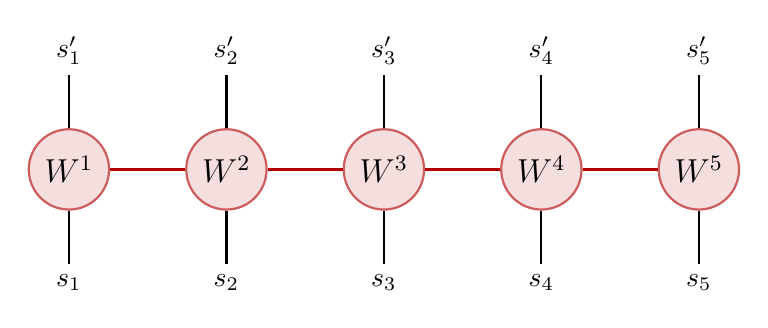
\begin{tikzpicture}[scale=1]
    \foreach \x/\label in {0/1, 2/2, 4/3, 6/4, 8/5} {
        \node[tensorR, minimum size=0.8cm] (W\label) at (\x, 0) {$W^{\label}$};
        \draw[leg] (W\label) -- ++(0,-1.2) node[below] {$s_{\label}$};
        \draw[leg] (W\label) -- ++(0,1.2) node[above] {$s'_{\label}$};
    }
    \draw[cleg] (W1) -- (W2);
    \draw[cleg] (W2) -- (W3);
    \draw[cleg] (W3) -- (W4);
    \draw[cleg] (W4) -- (W5);
\end{tikzpicture}
\caption{矩阵乘积算符（MPO）：每个张量有上下两个物理指标}
\end{figure}

\begin{examplebox}[例11：一维横场 Ising 模型的 MPO]
哈密顿量 $H = -J\sum_i \sigma^z_i \sigma^z_{i+1} - h\sum_i \sigma^x_i$ 可以写为 MPO，其中每个 $W$ 矩阵为：
\[
W = \begin{pmatrix} I & 0 & 0 \\ \sigma^z & 0 & 0 \\ -h\sigma^x & -J\sigma^z & I \end{pmatrix}
\]
这里每个矩阵元素本身是 $2\times 2$ 的算符矩阵，所以 $W$ 的键维度为 $D_W = 3$。
\end{examplebox}

\subsection{MPO 作用在 MPS 上}

将 MPO 作用在 MPS 上，就是将两层张量网络收缩：

\begin{figure}[H]
\centering
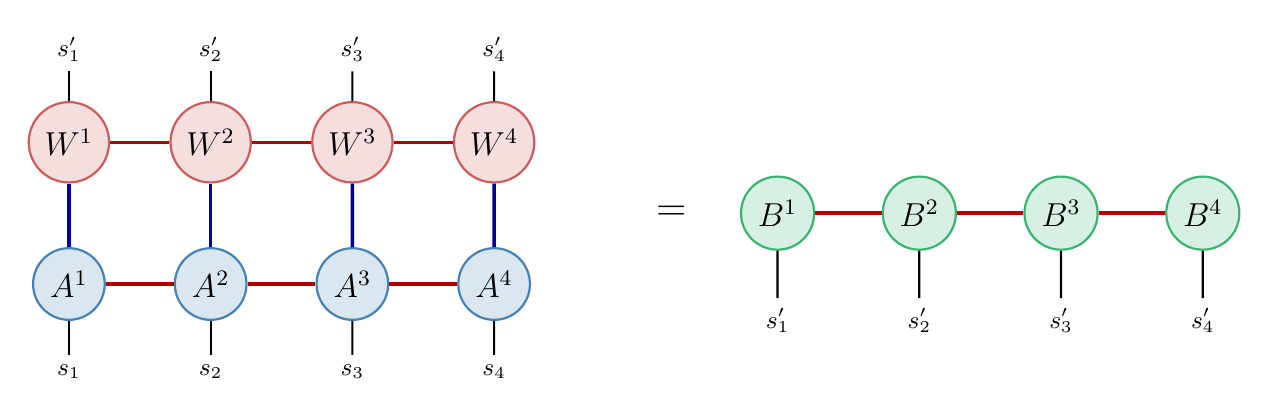
\begin{tikzpicture}[scale=0.9]
    % MPS layer
    \foreach \x/\label in {0/1, 2/2, 4/3, 6/4} {
        \node[tensor, minimum size=0.7cm] (A\label) at (\x, -1.5) {$A^{\label}$};
        \draw[leg] (A\label) -- ++(0,-1) node[below, font=\small] {$s_{\label}$};
    }
    \draw[cleg] (A1) -- (A2);
    \draw[cleg] (A2) -- (A3);
    \draw[cleg] (A3) -- (A4);

    % MPO layer
    \foreach \x/\label in {0/1, 2/2, 4/3, 6/4} {
        \node[tensorR, minimum size=0.7cm] (W\label) at (\x, 0.5) {$W^{\label}$};
        \draw[leg] (W\label) -- ++(0,1) node[above, font=\small] {$s'_{\label}$};
    }
    \draw[cleg] (W1) -- (W2);
    \draw[cleg] (W2) -- (W3);
    \draw[cleg] (W3) -- (W4);

    % Vertical connections
    \foreach \label in {1,2,3,4} {
        \draw[cleg, blue!60!black] (A\label) -- (W\label);
    }

    \node at (8.5, -0.5) {\Large $=$};

    % Result MPS
    \foreach \x/\label in {10/1, 12/2, 14/3, 16/4} {
        \node[tensorG, minimum size=0.7cm] (B\label) at (\x, -0.5) {$B^{\label}$};
        \draw[leg] (B\label) -- ++(0,-1.2) node[below, font=\small] {$s'_{\label}$};
    }
    \draw[cleg] (B1) -- (B2);
    \draw[cleg] (B2) -- (B3);
    \draw[cleg] (B3) -- (B4);
\end{tikzpicture}
\caption{MPO 作用在 MPS 上：垂直的腿被收缩，结果是新的 MPS（键维度为 $D \times D_W$）}
\end{figure}

\subsection{PEPS：二维张量网络}

\textbf{射影纠缠对态}（Projected Entangled Pair States，PEPS）是 MPS 到二维的自然推广。在二维方格子上，每个张量有一个物理指标和四个键指标（上下左右）：

\begin{figure}[H]
\centering
\begin{tikzpicture}[scale=1]
    \foreach \x in {0,2,4} {
        \foreach \y in {0,2,4} {
            \node[tensor, minimum size=0.6cm, font=\small] (t\x\y) at (\x, \y) {};
        }
    }
    % Horizontal bonds
    \foreach \y in {0,2,4} {
        \draw[cleg] (t0\y) -- (t2\y);
        \draw[cleg] (t2\y) -- (t4\y);
    }
    % Vertical bonds
    \foreach \x in {0,2,4} {
        \draw[cleg] (t\x 0) -- (t\x 2);
        \draw[cleg] (t\x 2) -- (t\x 4);
    }
    % Physical legs (going into the page, shown as dots)
    \foreach \x in {0,2,4} {
        \foreach \y in {0,2,4} {
            \draw[leg, gray] (t\x\y) -- ++(-0.5,-0.5);
        }
    }
    \node at (2,-1.2) {物理指标（向纸面外）};
\end{tikzpicture}
\caption{PEPS：二维方格子上的张量网络}
\end{figure}

PEPS 可以表示满足二维面积律的态，但其收缩（计算期望值等）通常是 \#P-hard 的，需要近似方法。

\subsection{树张量网络（TTN）}

\textbf{树张量网络}（Tree Tensor Network，TTN）具有树状的层次结构，没有环路：

\begin{figure}[H]
\centering
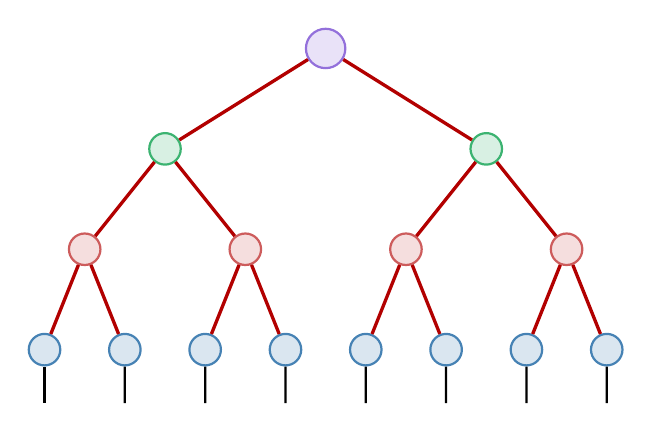
\begin{tikzpicture}[scale=0.85]
    % Bottom layer (physical)
    \foreach \x in {0,1,2,3,4,5,6,7} {
        \node[tensor, minimum size=0.4cm] (p\x) at (\x*1.2, 0) {};
        \draw[leg] (p\x) -- ++(0,-0.8);
    }
    % Second layer
    \foreach \x/\i in {0/0, 1/1, 2/2, 3/3} {
        \pgfmathsetmacro{\xpos}{\x*2.4+0.6}
        \node[tensorR, minimum size=0.4cm] (s\x) at (\xpos, 1.5) {};
        \pgfmathsetmacro{\left}{int(\x*2)}
        \pgfmathsetmacro{\right}{int(\x*2+1)}
        \draw[cleg] (s\x) -- (p\left);
        \draw[cleg] (s\x) -- (p\right);
    }
    % Third layer
    \foreach \x in {0,1} {
        \pgfmathsetmacro{\xpos}{\x*4.8+1.8}
        \node[tensorG, minimum size=0.4cm] (th\x) at (\xpos, 3) {};
        \pgfmathsetmacro{\left}{int(\x*2)}
        \pgfmathsetmacro{\right}{int(\x*2+1)}
        \draw[cleg] (th\x) -- (s\left);
        \draw[cleg] (th\x) -- (s\right);
    }
    % Top
    \node[tensorP, minimum size=0.5cm] (top) at (4.2, 4.5) {};
    \draw[cleg] (top) -- (th0);
    \draw[cleg] (top) -- (th1);
\end{tikzpicture}
\caption{树张量网络（TTN）：层次化的二叉树结构}
\end{figure}

TTN 的优点是收缩非常高效（从叶子到根逐层收缩），但它不如 MPS 那样适合描述具有平移不变性的一维系统。

\subsection{MERA：多尺度纠缠重正化}

\textbf{多尺度纠缠重正化 Ansatz}（Multiscale Entanglement Renormalization Ansatz，MERA）在树张量网络的基础上加入了\textbf{解纠缠器}（disentangler），使其能描述\textbf{临界系统}（纠缠熵随系统大小对数增长）。

\begin{figure}[H]
\centering
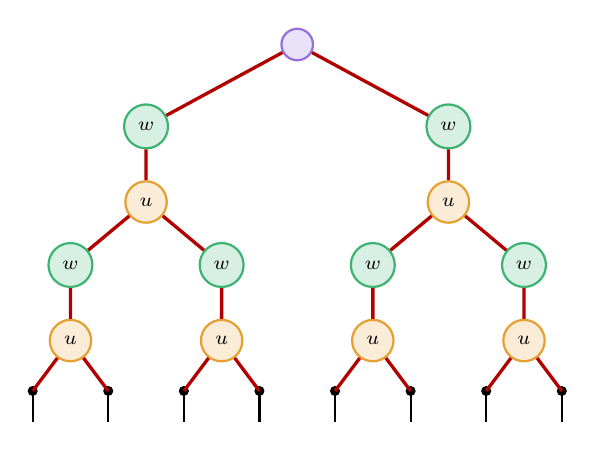
\begin{tikzpicture}[scale=0.8]
    % Physical sites
    \foreach \x in {0,...,7} {
        \draw[fill=black] (\x*1.2, 0) circle (2pt);
        \draw[leg] (\x*1.2, 0) -- ++(0, -0.5);
    }
    % Disentanglers (layer 1)
    \foreach \x in {0,1,2,3} {
        \pgfmathsetmacro{\xp}{\x*2.4+0.6}
        \node[tensorO, minimum size=0.35cm, font=\scriptsize] (d1\x) at (\xp, 0.8) {$u$};
        \pgfmathsetmacro{\left}{\x*2*1.2}
        \pgfmathsetmacro{\right}{(\x*2+1)*1.2}
        \draw[cleg] (d1\x) -- (\left, 0);
        \draw[cleg] (d1\x) -- (\right, 0);
    }
    % Isometries (layer 1)
    \foreach \x in {0,1,2,3} {
        \pgfmathsetmacro{\xp}{\x*2.4+0.6}
        \node[tensorG, minimum size=0.35cm, font=\scriptsize] (w1\x) at (\xp, 2) {$w$};
        \draw[cleg] (w1\x) -- (d1\x);
    }
    % Disentanglers (layer 2)
    \foreach \x in {0,1} {
        \pgfmathsetmacro{\xp}{\x*4.8+1.8}
        \node[tensorO, minimum size=0.35cm, font=\scriptsize] (d2\x) at (\xp, 3) {$u$};
        \pgfmathsetmacro{\left}{int(\x*2)}
        \pgfmathsetmacro{\right}{int(\x*2+1)}
        \draw[cleg] (d2\x) -- (w1\left);
        \draw[cleg] (d2\x) -- (w1\right);
    }
    % Isometries (layer 2)
    \foreach \x in {0,1} {
        \pgfmathsetmacro{\xp}{\x*4.8+1.8}
        \node[tensorG, minimum size=0.35cm, font=\scriptsize] (w2\x) at (\xp, 4.2) {$w$};
        \draw[cleg] (w2\x) -- (d2\x);
    }
    % Top
    \node[tensorP, minimum size=0.4cm] (top) at (4.2, 5.5) {};
    \draw[cleg] (top) -- (w20);
    \draw[cleg] (top) -- (w21);
\end{tikzpicture}
\caption{MERA：交替排列解纠缠器 $u$ 和等距映射 $w$}
\end{figure}

%=============================================================
\section{张量收缩的实践}
%=============================================================

\subsection{收缩顺序至关重要}

当一个张量网络包含三个或更多张量时，收缩的\textbf{顺序}对计算效率有巨大影响。

\begin{examplebox}[例12：收缩顺序的影响（矩阵链乘法）]
考虑三个矩阵 $A$（$2\times 100$）、$B$（$100\times 100$）、$C$（$100\times 3$）的乘积 $ABC$。

\textbf{方案一}：先算 $AB$，再乘 $C$
\begin{itemize}
    \item $AB$：$2\times 100 \times 100 = 20000$ 次乘法，结果是 $2\times 100$
    \item $(AB)C$：$2\times 100 \times 3 = 600$ 次乘法
    \item 总计：$20{,}600$ 次
\end{itemize}

\textbf{方案二}：先算 $BC$，再乘 $A$
\begin{itemize}
    \item $BC$：$100\times 100 \times 3 = 30000$ 次乘法，结果是 $100\times 3$
    \item $A(BC)$：$2\times 100 \times 3 = 600$ 次乘法
    \item 总计：$30{,}600$ 次
\end{itemize}

两种顺序的计算量相差约 50\%！对于更大的张量网络，差异可以是指数级的。
\end{examplebox}

\begin{examplebox}[例13：收缩顺序的指数级差异]
考虑一个环形张量网络，由 $N$ 个 $D\times D$ 矩阵 $M_1, M_2, \ldots, M_N$ 相乘并取迹：
\[
\text{tr}(M_1 M_2 \cdots M_N)
\]

\textbf{好的顺序}：从左到右依次收缩，每步都是 $D\times D$ 矩阵乘 $D\times D$ 矩阵。
\begin{itemize}
    \item 每步复杂度 $O(D^3)$，共 $N-1$ 步
    \item 总计 $O(ND^3)$ —— \textbf{多项式！}
\end{itemize}

\textbf{坏的顺序}：如果我们试图先把所有矩阵"张开"再收缩（不按顺序），中间结果可能变成高阶张量，复杂度可达 $O(D^N)$ —— \textbf{指数级！}
\end{examplebox}

\subsection{收缩顺序的一般原则}

\begin{keybox}[收缩的黄金法则]
\begin{enumerate}
    \item \textbf{先收缩小维度的指标}：优先消去维度小的指标
    \item \textbf{避免产生高阶中间张量}：尽量让中间结果的阶数不要太大
    \item \textbf{利用网络结构}：树状网络从叶子向根收缩；链状网络（MPS）从一端向另一端收缩
    \item \textbf{最优收缩顺序}通常是一个NP-hard问题（等价于"最优矩阵链乘法"的推广），但有很好的启发式算法
\end{enumerate}
\end{keybox}

\subsection{MPS 的逐步收缩示例}

让我们通过一个完整的例子，展示如何收缩一个 MPS 来计算量子态的某个分量。

\begin{examplebox}[例14：手动收缩一个三格点 MPS]
考虑一个三格点的 MPS（每个物理指标维度 $d=2$，键维度 $D=2$）：

格点1的张量 $A^{s_1}$（$1\times 2$ 矩阵，因为左边界）：
\[
A^{0} = \begin{pmatrix} 1 & 0 \end{pmatrix}, \quad A^{1} = \begin{pmatrix} 0 & 1 \end{pmatrix}
\]

格点2的张量 $B^{s_2}$（$2\times 2$ 矩阵）：
\[
B^{0} = \begin{pmatrix} 1 & 1 \\ 0 & 0 \end{pmatrix}, \quad B^{1} = \begin{pmatrix} 0 & 0 \\ 1 & 1 \end{pmatrix}
\]

格点3的张量 $C^{s_3}$（$2\times 1$ 矩阵，因为右边界）：
\[
C^{0} = \begin{pmatrix} 1 \\ 0 \end{pmatrix}, \quad C^{1} = \begin{pmatrix} 0 \\ 1 \end{pmatrix}
\]

计算 $\ket{010}$ 的系数 $\Psi_{010}$：
\begin{align}
\Psi_{010} &= A^0 B^1 C^0 \\
&= \begin{pmatrix} 1 & 0 \end{pmatrix}
\begin{pmatrix} 0 & 0 \\ 1 & 1 \end{pmatrix}
\begin{pmatrix} 1 \\ 0 \end{pmatrix} \\
&= \begin{pmatrix} 0 & 0 \end{pmatrix}
\begin{pmatrix} 1 \\ 0 \end{pmatrix} \\
&= 0
\end{align}

计算 $\ket{100}$ 的系数 $\Psi_{100}$：
\begin{align}
\Psi_{100} &= A^1 B^0 C^0
= \begin{pmatrix} 0 & 1 \end{pmatrix}
\begin{pmatrix} 1 & 1 \\ 0 & 0 \end{pmatrix}
\begin{pmatrix} 1 \\ 0 \end{pmatrix}
= \begin{pmatrix} 0 & 0 \end{pmatrix}
\begin{pmatrix} 1 \\ 0 \end{pmatrix} = 0
\end{align}

计算 $\ket{110}$ 的系数：
\begin{align}
\Psi_{110} &= A^1 B^1 C^0
= \begin{pmatrix} 0 & 1 \end{pmatrix}
\begin{pmatrix} 0 & 0 \\ 1 & 1 \end{pmatrix}
\begin{pmatrix} 1 \\ 0 \end{pmatrix}
= \begin{pmatrix} 1 & 1 \end{pmatrix}
\begin{pmatrix} 1 \\ 0 \end{pmatrix} = 1
\end{align}

读者可以验证，这个 MPS 表示的态为 $\ket{\Psi} = \ket{001} + \ket{011} + \ket{110} + \ket{111}$（未归一化）。
\end{examplebox}

\subsection{计算期望值：$\langle\Psi|\hat{O}|\Psi\rangle$ 的收缩}

MPS 最常见的应用之一是计算期望值。对于一个单格点算符 $\hat{O}$ 作用在第 $k$ 个格点上：

\begin{equation}
\langle\Psi|\hat{O}_k|\Psi\rangle =
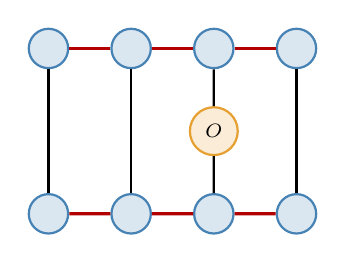
\begin{tikzpicture}[baseline=(current bounding box.center), scale=0.7]
    % Bra
    \foreach \x/\label in {0/1, 1.5/2, 3/3, 4.5/4} {
        \node[tensor, minimum size=0.5cm, font=\scriptsize] (A\label) at (\x, 0) {};
    }
    \draw[cleg] (A1) -- (A2);
    \draw[cleg] (A2) -- (A3);
    \draw[cleg] (A3) -- (A4);

    % Ket
    \foreach \x/\label in {0/1, 1.5/2, 3/3, 4.5/4} {
        \node[tensor, minimum size=0.5cm, font=\scriptsize] (B\label) at (\x, -3) {};
    }
    \draw[cleg] (B1) -- (B2);
    \draw[cleg] (B2) -- (B3);
    \draw[cleg] (B3) -- (B4);

    % Operator
    \node[tensorO, minimum size=0.5cm, font=\scriptsize] (O) at (3, -1.5) {$O$};

    % Vertical connections
    \draw[leg] (A1) -- (B1);
    \draw[leg] (A2) -- (B2);
    \draw[leg] (A3) -- (O);
    \draw[leg] (O) -- (B3);
    \draw[leg] (A4) -- (B4);
\end{tikzpicture}
\end{equation}

收缩策略：\textbf{从左向右}，逐步将上下两层的张量收缩成一个"转移矩阵"。

%=============================================================
\section{张量分解方法}
%=============================================================

张量网络不仅用于\textbf{表示}量子态，还需要\textbf{构建}和\textbf{优化}。这依赖于几种关键的张量分解方法。

\subsection{奇异值分解（SVD）}

SVD 是张量网络中最重要的工具。对于矩阵 $M$（$m \times n$）：
\begin{equation}
    M = U \Sigma V^\dagger
\end{equation}
其中 $U$（$m\times r$）和 $V$（$n\times r$）是等距矩阵，$\Sigma$（$r\times r$）是对角矩阵，对角元素 $\sigma_1 \geq \sigma_2 \geq \cdots \geq 0$ 是奇异值。

\begin{figure}[H]
\centering
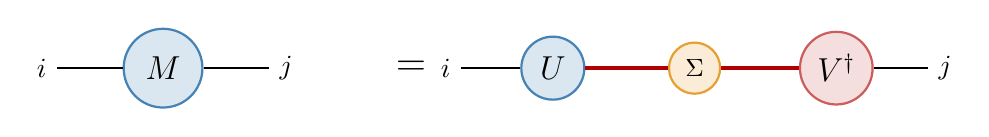
\begin{tikzpicture}[scale=0.9]
    \node[tensor, minimum size=1cm] (M) at (0,0) {$M$};
    \draw[leg] (M) -- ++(-1.5,0) node[left] {$i$};
    \draw[leg] (M) -- ++(1.5,0) node[right] {$j$};

    \node at (3.5,0) {\Large $=$};

    \node[tensor, minimum size=0.8cm] (U) at (5.5,0) {$U$};
    \node[tensorO, minimum size=0.6cm, font=\small] (S) at (7.5,0) {$\Sigma$};
    \node[tensorR, minimum size=0.8cm] (V) at (9.5,0) {$V^\dagger$};
    \draw[leg] (U) -- ++(-1.3,0) node[left] {$i$};
    \draw[cleg] (U) -- (S);
    \draw[cleg] (S) -- (V);
    \draw[leg] (V) -- ++(1.3,0) node[right] {$j$};
\end{tikzpicture}
\caption{SVD 的图形表示}
\end{figure}

\begin{examplebox}[例15：SVD 与截断]
考虑矩阵 $M = \begin{pmatrix} 3 & 0 \\ 0 & 1 \\ 0 & 0 \end{pmatrix}$。

SVD：$U = \begin{pmatrix} 1 & 0 \\ 0 & 1 \\ 0 & 0\end{pmatrix}$，$\Sigma = \begin{pmatrix} 3 & 0 \\ 0 & 1\end{pmatrix}$，$V^\dagger = \begin{pmatrix} 1 & 0 \\ 0 & 1\end{pmatrix}$。

如果我们只保留最大的奇异值 $\sigma_1 = 3$（\textbf{截断}到 $D=1$）：
\[
M \approx \tilde{M} = \begin{pmatrix} 1 \\ 0 \\ 0\end{pmatrix} (3) \begin{pmatrix} 1 & 0 \end{pmatrix} = \begin{pmatrix} 3 & 0 \\ 0 & 0 \\ 0 & 0 \end{pmatrix}
\]

截断误差：$\|M - \tilde{M}\|_F = \sigma_2 = 1$。

Eckart--Young 定理保证：SVD 截断是最优的低秩近似。
\end{examplebox}

\subsection{将高阶张量分解为 MPS}

通过反复应用 SVD，可以将任何高阶张量分解为 MPS。

\begin{examplebox}[例16：用 SVD 将四阶张量变为 MPS]
给定四阶张量 $T_{s_1 s_2 s_3 s_4}$（所有指标维度 $d=2$，共 $2^4 = 16$ 个分量）。

\textbf{步骤1}：把 $T$ 看作矩阵 $M^{(1)}_{s_1, (s_2 s_3 s_4)}$（$2 \times 8$ 矩阵），做 SVD：
\[
T_{s_1, (s_2 s_3 s_4)} = \sum_{\alpha_1} U^{(1)}_{s_1, \alpha_1} \, \Sigma^{(1)}_{\alpha_1} \, V^{(1)\dagger}_{\alpha_1, (s_2 s_3 s_4)}
\]
将 $\Sigma V^\dagger$ 合并，$A^{(1)}_{s_1, \alpha_1} = U^{(1)}_{s_1, \alpha_1}$，剩余部分为 $R_{\alpha_1, s_2 s_3 s_4}$。

\textbf{步骤2}：把 $R$ 重塑为矩阵 $M^{(2)}_{(\alpha_1 s_2), (s_3 s_4)}$，做 SVD：
\[
R_{(\alpha_1 s_2), (s_3 s_4)} = \sum_{\alpha_2} U^{(2)}_{(\alpha_1 s_2), \alpha_2} \, \Sigma^{(2)}_{\alpha_2} \, V^{(2)\dagger}_{\alpha_2, (s_3 s_4)}
\]
得到 $A^{(2)}_{\alpha_1, s_2, \alpha_2}$。

\textbf{步骤3}：对剩余部分重复，得到 $A^{(3)}_{\alpha_2, s_3, \alpha_3}$ 和 $A^{(4)}_{\alpha_3, s_4}$。

最终：$T_{s_1 s_2 s_3 s_4} = \sum_{\alpha_1, \alpha_2, \alpha_3} A^{(1)}_{s_1, \alpha_1} A^{(2)}_{\alpha_1, s_2, \alpha_2} A^{(3)}_{\alpha_2, s_3, \alpha_3} A^{(4)}_{\alpha_3, s_4}$

如果在每步 SVD 时截断到最大键维度 $D$，就得到了一个近似的 MPS。
\end{examplebox}

\subsection{QR 分解}

QR 分解也常用于张量网络算法中（特别是在正则化 MPS 时）：
\begin{equation}
    M = QR
\end{equation}
其中 $Q$ 是等距矩阵（$Q^\dagger Q = I$），$R$ 是上三角矩阵。

QR 比 SVD 快，但不提供奇异值信息，因此不能用于截断。

%=============================================================
\section{张量网络算法}
%=============================================================

\subsection{DMRG：密度矩阵重正化群}

\textbf{DMRG}（Density Matrix Renormalization Group）是张量网络最成功的算法之一，由 Steven White 于 1992 年提出。它本质上是在 MPS 变分空间中寻找哈密顿量基态。

\begin{keybox}[DMRG 的基本思想]
\begin{enumerate}
    \item 将量子态表示为 MPS
    \item 固定其他格点的张量，优化一个（或两个相邻）格点的张量
    \item 从左到右、再从右到左反复扫描（sweep）
    \item 每步优化等价于一个标准特征值问题
    \item 直到能量收敛
\end{enumerate}
\end{keybox}

DMRG 的优化过程可以用张量网络图形直观理解：

\begin{figure}[H]
\centering
\begin{tikzpicture}[scale=0.8]
    % Environment (left)
    \node[tensorG, minimum size=0.7cm, font=\small] (L) at (0, -1) {$L$};

    % Optimized tensor
    \node[tensorR, minimum size=0.9cm] (A) at (2.5, 0) {$A^*$};
    \draw[leg] (A) -- ++(0,1.2) node[above] {$s_k$};

    % MPO
    \node[tensorO, minimum size=0.7cm, font=\small] (W) at (2.5, -2) {$W_k$};

    % Environment (right)
    \node[tensorG, minimum size=0.7cm, font=\small] (R) at (5, -1) {$R$};

    % Connections
    \draw[cleg] (L) -- ++(0,1) -| (A);
    \draw[cleg] (L) -- (W);
    \draw[cleg] (L) -- ++(0,-1) -| (2.5, -3.5) -- ++(0,0);
    \draw[cleg] (W) -- (R);
    \draw[cleg] (A) -| (R |- 0,0) -- (R);
    \draw[cleg] (R) -- ++(0,-1) -- ++(-2.5, 0) -- ++(0,0.5);
    \draw[leg] (W) -- ++(0,-1.5) node[below] {$s'_k$};
    \draw[leg] (A) -- (W);

    \node at (7, -1) {\Large $\Rightarrow$};
    \node[align=left, font=\small] at (10, -1) {求解有效\\特征值问题\\$H_{\text{eff}} A^* = E A^*$};
\end{tikzpicture}
\caption{DMRG 单格点优化示意：环境张量 $L$ 和 $R$ 包含了左右两侧的信息}
\end{figure}

\begin{examplebox}[例17：DMRG 求解一维 Heisenberg 模型]
考虑反铁磁 Heisenberg 链：
\[
H = J\sum_i \vec{S}_i \cdot \vec{S}_{i+1} = J\sum_i \left(S^x_i S^x_{i+1} + S^y_i S^y_{i+1} + S^z_i S^z_{i+1}\right)
\]
对于 $N=100$ 个 spin-1/2，DMRG 用 $D \sim 100{-}200$ 的 MPS 就能将基态能量精确到 $10^{-10}$ 的相对误差。这是精确对角化（只能处理 $N \sim 20$）无法企及的。
\end{examplebox}

\subsection{时间演化算法（TEBD）}

\textbf{TEBD}（Time-Evolving Block Decimation）用于模拟量子态的时间演化：
\begin{equation}
    \ket{\Psi(t)} = e^{-iHt}\ket{\Psi(0)}
\end{equation}

核心思想是 Trotter 分解：
\begin{equation}
    e^{-iH\delta t} \approx e^{-iH_{\text{odd}}\delta t} e^{-iH_{\text{even}}\delta t} + O(\delta t^2)
\end{equation}
其中 $H_{\text{odd/even}}$ 分别包含奇数/偶数位置的近邻相互作用。每个 $e^{-ih_{i,i+1}\delta t}$ 是一个两格点门，可以直接作用在 MPS 上。

\begin{figure}[H]
\centering
\begin{tikzpicture}[scale=0.7]
    % MPS
    \foreach \x/\name in {0/a1, 1.5/a2, 3/a3, 4.5/a4, 6/a5, 7.5/a6} {
        \node[tensor, minimum size=0.5cm] (\name) at (\x, 0) {};
        \draw[leg] (\name) -- ++(0, -0.8);
    }
    \draw[cleg] (a1) -- (a2);
    \draw[cleg] (a2) -- (a3);
    \draw[cleg] (a3) -- (a4);
    \draw[cleg] (a4) -- (a5);
    \draw[cleg] (a5) -- (a6);

    % Even gates
    \foreach \x/\gname in {0/g1, 3/g2, 6/g3} {
        \pgfmathsetmacro{\xr}{\x+1.5}
        \node[tensorO, minimum size=0.4cm, rectangle, minimum width=1.8cm, font=\scriptsize] (\gname) at (\x+0.75, -1.5) {$e^{-ih\delta t}$};
        \draw[leg] (\gname.north west) ++(0.15,0) -- ++(0, 0.7);
        \draw[leg] (\gname.north east) ++(-0.15,0) -- ++(0, 0.7);
    }

    \node[font=\small] at (3.75, -2.5) {偶数格点门};
\end{tikzpicture}
\caption{TEBD 的一个 Trotter 步：两格点门作用在 MPS 上}
\end{figure}

每次作用一个两格点门后，需要用 SVD 截断将键维度控制在 $D$ 以内，这是 TEBD 的近似所在。

%=============================================================
\section{张量收缩的进阶话题}
%=============================================================

\subsection{张量网络的收缩复杂度}

不同网络结构的收缩难度差别很大：

\begin{table}[H]
\centering
\begin{tabular}{lcc}
\toprule
\textbf{网络类型} & \textbf{精确收缩} & \textbf{复杂度} \\
\midrule
MPS（一维链） & 可以 & $O(ND^3 d)$ \\
TTN（树） & 可以 & $O(ND^4)$ \\
MERA & 可以 & $O(ND^8)$（typical） \\
PEPS（二维） & \#P-hard & 需要近似方法 \\
一般图 & \#P-hard & NP-hard（最优顺序） \\
\bottomrule
\end{tabular}
\caption{不同张量网络结构的收缩复杂度}
\end{table}

\subsection{近似收缩方法}

对于无法精确收缩的张量网络（如 PEPS），常用的近似方法包括：

\begin{enumerate}
    \item \textbf{边界 MPS 方法}：用一个 MPS 来近似表示张量网络的部分收缩结果。逐行收缩二维网络时，用 MPS 近似每一行收缩后的结果。

    \item \textbf{角转移矩阵法}（Corner Transfer Matrix, CTM）：利用角转移矩阵来近似无穷大 PEPS 的环境。

    \item \textbf{张量重正化群}（TRG, Tensor Renormalization Group）：通过反复对张量做 SVD 分解和重组，粗粒化张量网络。
\end{enumerate}

\begin{examplebox}[例18：TRG 的基本思想]
考虑二维经典 Ising 模型的配分函数，可以表示为一个二维张量网络。TRG 的步骤：

\textbf{步骤1}：对每个四阶张量 $T_{ijkl}$ 做 SVD 分解：
\[
T_{ijkl} = \sum_\alpha S^{(1)}_{ij\alpha} S^{(2)}_{kl\alpha}
\]

\textbf{步骤2}：重新组合相邻的半张量，形成新的四阶张量 $T'$。

\textbf{步骤3}：新的张量网络格点数减半，重复以上步骤。

每次粗粒化将格点数减少一半，$\log_2 N$ 步后，整个网络被收缩为一个数（配分函数）。
\end{examplebox}

\subsection{自动微分与张量网络}

近年来，\textbf{自动微分}（automatic differentiation）被引入张量网络计算中。这使得我们可以：
\begin{itemize}
    \item 自动计算张量网络中参数的梯度
    \item 使用梯度下降等优化方法来优化张量网络
    \item 将张量网络与机器学习框架（如 PyTorch, JAX）结合
\end{itemize}

%=============================================================
\section{张量网络的应用}
%=============================================================

\subsection{量子多体物理}

张量网络最重要的应用是在量子多体物理中：

\begin{itemize}
    \item \textbf{基态搜索}：DMRG 是求解一维量子系统基态的"金标准"方法
    \item \textbf{时间演化}：TEBD, tDMRG 等方法模拟量子动力学
    \item \textbf{有限温度}：利用虚时间演化或 purification 方法研究热力学性质
    \item \textbf{二维系统}：iPEPS + CTM 方法用于研究二维量子系统
\end{itemize}

\begin{examplebox}[例19：DMRG 在一维系统中的经典应用]
\begin{itemize}
    \item \textbf{Haldane 猜想验证}：DMRG 精确计算了 spin-1 Heisenberg 链的 Haldane 能隙
    \item \textbf{Hubbard 模型}：一维 Hubbard 模型的精确基态和关联函数
    \item \textbf{量子相变}：通过纠缠熵的标度行为识别量子临界点
\end{itemize}
\end{examplebox}

\subsection{经典统计力学}

二维经典统计模型的配分函数可以自然地表示为张量网络：

\begin{examplebox}[例20：二维 Ising 模型的张量网络表示]
考虑二维方格子 Ising 模型：
\[
Z = \sum_{\{s\}} \prod_{\langle ij \rangle} e^{\beta J s_i s_j}
\]
其中 $s_i = \pm 1$。

对每个格点定义四阶张量 $T_{udlr}$（上下左右指标各维度2）：
\[
T_{udlr} = \sum_{s=\pm 1} W_{su} W_{sd} W_{sl} W_{sr}
\]
其中 $W_{s,s'} = e^{\frac{\beta J}{4} s s'}$。

这样，配分函数就等于所有张量的完全收缩：
\[
Z = \text{tTr}\left(\prod T\right)
\]
这就是一个二维张量网络！可以用 TRG 或 CTM 等方法来近似计算。
\end{examplebox}

\subsection{量子计算}

量子电路可以自然地表示为张量网络：
\begin{itemize}
    \item 每个量子门是一个张量
    \item 量子比特的演化对应张量的连接
    \item 模拟量子电路等价于收缩对应的张量网络
\end{itemize}

\begin{figure}[H]
\centering
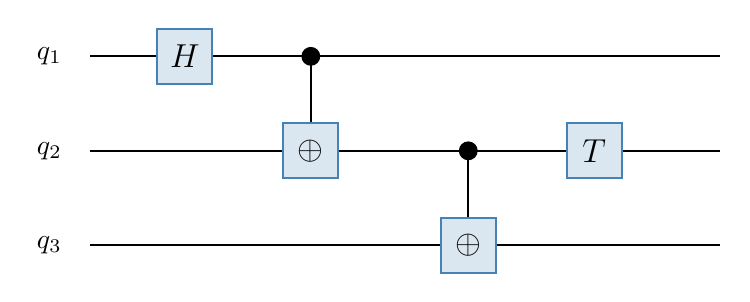
\begin{tikzpicture}[scale=0.8]
    % Qubits
    \foreach \y/\label in {0/q_3, 1.5/q_2, 3/q_1} {
        \draw[thick] (0, \y) -- (10, \y);
        \node[left] at (-0.3, \y) {$\label$};
    }

    % Single qubit gates
    \node[tensorS, minimum size=0.7cm] (H1) at (1.5, 3) {$H$};
    \node[tensorS, minimum size=0.7cm] (T1) at (8, 1.5) {$T$};

    % CNOT
    \draw[fill=black] (3.5, 3) circle (4pt);
    \draw[thick] (3.5, 3) -- (3.5, 1.5);
    \node[tensorS, minimum size=0.7cm] (X1) at (3.5, 1.5) {$\oplus$};

    % Another CNOT
    \draw[fill=black] (6, 1.5) circle (4pt);
    \draw[thick] (6, 1.5) -- (6, 0);
    \node[tensorS, minimum size=0.7cm] (X2) at (6, 0) {$\oplus$};
\end{tikzpicture}
\caption{量子电路本质上就是一种张量网络}
\end{figure}

\subsection{机器学习中的张量网络}

张量网络方法也被应用到机器学习中：
\begin{itemize}
    \item \textbf{张量训练分解}（Tensor Train, TT）：MPS 在数值分析中的别名，用于高维函数逼近
    \item \textbf{模型压缩}：用 TT 分解压缩神经网络的权重张量
    \item \textbf{生成模型}：MPS/PEPS 作为概率分布的参数化，用于无监督学习
    \item \textbf{特征映射}：将数据映射到高维空间后用张量网络进行分类
\end{itemize}

%=============================================================
\section{数值实例：用 Python 实现张量收缩}
%=============================================================

为了加深理解，本节展示如何用简单的代码实现张量收缩。即使你不熟悉编程，阅读这些伪代码也有助于理解收缩的机制。

\subsection{用循环实现矩阵乘法}

矩阵乘法 $C_{ij} = \sum_k A_{ik} B_{kj}$ 的最直接实现：

\begin{tcolorbox}[colback=gray!5, colframe=gray!60, fonttitle=\bfseries, title=矩阵乘法的显式循环实现]
\begin{verbatim}
# A: m x p 矩阵, B: p x n 矩阵
# C: m x n 矩阵 (结果)
for i in range(m):
    for j in range(n):
        C[i,j] = 0
        for k in range(p):       # 对收缩指标 k 求和
            C[i,j] += A[i,k] * B[k,j]
\end{verbatim}
\end{tcolorbox}

注意三重循环对应三个指标 $i, j, k$，其中 $k$ 是被收缩的指标。

\subsection{用 \texttt{einsum} 表示张量收缩}

现代数值库（如 NumPy）提供了 \texttt{einsum} 函数，它用 Einstein 求和约定来表达任意的张量收缩：

\begin{tcolorbox}[colback=gray!5, colframe=gray!60, fonttitle=\bfseries, title=用 einsum 实现各种张量收缩]
\begin{verbatim}
import numpy as np

# 向量内积: c = sum_i u_i v_i
c = np.einsum('i,i->', u, v)

# 矩阵乘法: C_ij = sum_k A_ik B_kj
C = np.einsum('ik,kj->ij', A, B)

# 矩阵的迹: c = sum_i A_ii
c = np.einsum('ii->', A)

# 三阶张量与矩阵收缩:
# D_ijl = sum_k T_ijk M_kl
D = np.einsum('ijk,kl->ijl', T, M)

# MPS 收缩 (三个格点):
# Psi_s1s2s3 = sum_{a1,a2} A_s1a1 B_a1s2a2 C_a2s3
Psi = np.einsum('ia,ajb,bk->ijk', A, B, C)
\end{verbatim}
\end{tcolorbox}

\begin{examplebox}[例21：用 einsum 计算 MPS 的内积]
两个 MPS $\ket{\Psi}$ 和 $\ket{\Phi}$ 的内积 $\langle\Phi|\Psi\rangle$ 可以通过逐步收缩来计算：

\begin{verbatim}
# 从左到右逐步收缩
# E: 转移矩阵的累积，初始为 1x1 单位矩阵
E = np.ones((1,1))
for n in range(N):
    # E_ab, A_asc, B_bsc -> E'_cd
    # 对物理指标 s 和左键指标 a,b 求和
    E = np.einsum('ab,asc,bsc->cd', E,
                   A_conj[n], B[n])
# 最终 E 是一个标量（1x1矩阵）
overlap = E[0,0]
\end{verbatim}

每步的复杂度为 $O(D^2 \cdot D \cdot d) = O(D^3 d)$，共 $N$ 步，总复杂度 $O(ND^3 d)$。
\end{examplebox}

\subsection{收缩顺序优化的数值实验}

\begin{examplebox}[例22：用 \texttt{opt\_einsum} 自动优化收缩顺序]
对于复杂的张量网络，手动确定最优收缩顺序非常困难。\texttt{opt\_einsum} 库可以自动找到（近似）最优顺序：

\begin{verbatim}
import opt_einsum as oe

# 定义一个包含5个张量的收缩
# (具体例子：环形网络的迹)
expr = oe.contract_expression(
    'ij,jk,kl,lm,mi->',
    (D,D), (D,D), (D,D), (D,D), (D,D),
    optimize='dp'  # 动态规划求最优顺序
)

# 查看优化后的计算量
path, info = oe.contract_path(
    'ij,jk,kl,lm,mi->', A, B, C, D, E,
    optimize='dp'
)
print(f"最优路径: {path}")
print(f"计算量: {info.opt_cost}")
\end{verbatim}
\end{examplebox}

%=============================================================
\section{Einstein 求和约定详解}
%=============================================================

Einstein 求和约定是张量计算中最常用的记号，也是理解 \texttt{einsum} 的基础。

\subsection{基本规则}

\begin{keybox}[Einstein 求和约定]
\begin{enumerate}
    \item 在一个表达式中，\textbf{重复出现}的指标表示对该指标\textbf{自动求和}
    \item 只出现一次的指标是\textbf{自由指标}，保留在结果中
    \item 求和号 $\sum$ 可以省略不写
\end{enumerate}
\end{keybox}

\begin{examplebox}[例23：Einstein 约定的各种用法]
\textbf{矩阵乘法}：
\[
C_{ij} = A_{ik} B_{kj} \quad \text{（省略了 $\sum_k$，因为 $k$ 出现了两次）}
\]

\textbf{矩阵的迹}：
\[
A_{ii} \equiv \sum_i A_{ii} = \text{tr}(A) \quad \text{（$i$ 出现两次，自动求和）}
\]

\textbf{向量内积}：
\[
u_i v_i \equiv \sum_i u_i v_i = \vec{u} \cdot \vec{v}
\]

\textbf{张量缩并}（自身指标收缩）：
\[
T_{iij} \equiv \sum_i T_{iij} \quad \text{（三阶张量变为一阶张量）}
\]

\textbf{多个指标的同时收缩}：
\[
A_{ij} B_{ji} \equiv \sum_i \sum_j A_{ij} B_{ji} = \text{tr}(AB)
\]
\end{examplebox}

\subsection{从 Einstein 约定到图形表示}

Einstein 约定和图形表示法是等价的两种语言：

\begin{table}[H]
\centering
\begin{tabular}{lll}
\toprule
\textbf{操作} & \textbf{Einstein 约定} & \textbf{图形表示} \\
\midrule
向量内积 & $u_i v_i$ & 两节点一条连线 \\
矩阵乘法 & $A_{ik} B_{kj}$ & 两节点一条连线，各余一条腿 \\
迹 & $A_{ii}$ & 一个节点两条腿自连 \\
外积 & $u_i v_j$ & 两节点无连线 \\
三张量链式收缩 & $A_{i\alpha} B_{\alpha j \beta} C_{\beta k}$ & 三节点串联 \\
\bottomrule
\end{tabular}
\caption{Einstein 约定与图形表示的对应关系}
\end{table}

%=============================================================
\section{正则形式与规范自由度}
%=============================================================

MPS 有一个重要特性：\textbf{规范自由度}（gauge freedom）。在任意两个相邻张量之间插入一对互逆矩阵 $X X^{-1} = I$，MPS 表示的物理态不变：

\begin{equation}
\cdots A^{s_n}_{\alpha_{n-1}\alpha_n} A^{s_{n+1}}_{\alpha_n \alpha_{n+1}} \cdots
= \cdots \tilde{A}^{s_n}_{\alpha_{n-1}\beta_n} \tilde{A}^{s_{n+1}}_{\beta_n \alpha_{n+1}} \cdots
\end{equation}
其中 $\tilde{A}^{s_n} = A^{s_n} X$，$\tilde{A}^{s_{n+1}} = X^{-1} A^{s_{n+1}}$。

\subsection{左正则与右正则形式}

利用规范自由度，可以将 MPS 变换为特殊的\textbf{正则形式}（canonical form）。

\begin{keybox}[正则条件]
\textbf{左正则}（left-canonical）：对于所有 $s_n$，
\[
\sum_{s_n} A^{s_n \dagger} A^{s_n} = I \quad \text{（等距条件）}
\]

\textbf{右正则}（right-canonical）：对于所有 $s_n$，
\[
\sum_{s_n} B^{s_n} B^{s_n \dagger} = I
\]
\end{keybox}

\begin{figure}[H]
\centering
\begin{tikzpicture}[scale=0.9]
    % Left canonical
    \node[tensor, minimum size=0.7cm] (A) at (0,0) {$A$};
    \node[tensor, minimum size=0.7cm, fill=tensorblue!40] (Ac) at (0, 1.8) {$A^*$};
    \draw[cleg] (A) -- ++(-1.2, 0);
    \draw[cleg] (Ac) -- ++(-1.2, 0);
    \draw[cleg] (A.east) -- ++(0.8,0);
    \draw[cleg] (Ac.east) -- ++(0.8,0);
    \draw[cleg] (A) -- (Ac) node[midway, right, font=\small] {$s$};

    \node at (2.5, 0.9) {\Large $=$};

    \draw[very thick] (3.8, 0) -- (3.8, 1.8);
    \node[right, font=\small] at (4, 0.9) {$= \delta_{\alpha\alpha'}$};

    % Label
    \node[below, font=\small] at (0, -0.8) {左正则条件};

    % Right canonical
    \node[tensorR, minimum size=0.7cm] (B) at (8,0) {$B$};
    \node[tensorR, minimum size=0.7cm, fill=tensorred!40] (Bc) at (8, 1.8) {$B^*$};
    \draw[cleg] (B) -- ++(1.2, 0);
    \draw[cleg] (Bc) -- ++(1.2, 0);
    \draw[cleg] (B.west) -- ++(-0.8,0);
    \draw[cleg] (Bc.west) -- ++(-0.8,0);
    \draw[cleg] (B) -- (Bc) node[midway, left, font=\small] {$s$};

    \node at (10.5, 0.9) {\Large $=$};

    \draw[very thick] (11.8, 0) -- (11.8, 1.8);
    \node[right, font=\small] at (12, 0.9) {$= \delta_{\beta\beta'}$};

    \node[below, font=\small] at (8, -0.8) {右正则条件};
\end{tikzpicture}
\caption{左正则和右正则条件的图形表示：收缩物理指标和一侧的键指标后得到单位矩阵}
\end{figure}

\subsection{混合正则形式与纠缠熵}

特别有用的是\textbf{混合正则形式}（mixed canonical form）：选定一个格点 $n$，使其左边的张量都是左正则的，右边的都是右正则的：

\begin{equation}
\ket{\Psi} = \sum A^{s_1} \cdots A^{s_{n-1}} \underbrace{\Lambda \Gamma^{s_n}}_{\text{中心张量}} B^{s_{n+1}} \cdots B^{s_N}
\end{equation}

在这种形式下，$\Lambda$ 的对角元素就是\textbf{纠缠谱}（entanglement spectrum），它们的平方给出 Schmidt 分解的系数。\textbf{纠缠熵}可以直接从中计算：
\begin{equation}
S = -\sum_\alpha \lambda_\alpha^2 \log \lambda_\alpha^2
\end{equation}

\begin{examplebox}[例24：从MPS读出纠缠熵]
设一个键上的 Schmidt 值为 $\lambda_1 = 0.9$，$\lambda_2 = 0.3$，$\lambda_3 = 0.1$（已归一化使 $\sum \lambda^2 = 1$ 后约为 $\lambda_1 \approx 0.943, \lambda_2 \approx 0.314, \lambda_3 \approx 0.105$）。

那么这个键的纠缠熵为：
\[
S = -(0.943^2 \ln 0.943^2 + 0.314^2 \ln 0.314^2 + 0.105^2 \ln 0.105^2) \approx 0.38
\]
最大可能的纠缠熵为 $\ln D = \ln 3 \approx 1.10$（当所有 $\lambda$ 相等时），所以这个态的纠缠不是最大的。
\end{examplebox}

%=============================================================
\section{张量网络与量子纠缠的几何图像}
%=============================================================

张量网络不仅是一种计算工具，更深刻地揭示了量子纠缠的\textbf{几何结构}。

\subsection{纠缠与几何的对应}

在张量网络中，纠缠结构由\textbf{网络的拓扑}决定：
\begin{itemize}
    \item 两个区域之间的纠缠上界 $\sim$ 连接这两个区域的键的数目 $\times \log D$
    \item MPS 中任意二分的最大纠缠为 $\log D$（只有一条键穿过切面）
    \item PEPS 中沿一条线切开，穿过的键数与线长成正比——自然满足面积律
\end{itemize}

\begin{figure}[H]
\centering
\begin{tikzpicture}[scale=0.8]
    % MPS with cut
    \foreach \x/\label in {0/1, 1.8/2, 3.6/3, 5.4/4, 7.2/5, 9/6} {
        \node[tensor, minimum size=0.6cm, font=\small] (a\label) at (\x, 0) {};
        \draw[leg] (a\label) -- ++(0,-0.8);
    }
    \draw[cleg] (a1) -- (a2);
    \draw[cleg] (a2) -- (a3);
    \draw[cleg] (a3) -- (a4);
    \draw[cleg] (a4) -- (a5);
    \draw[cleg] (a5) -- (a6);

    % Cut line
    \draw[dashed, thick, green!50!black] (4.5, -1.5) -- (4.5, 1) node[above, font=\small] {切割};

    % Arrow
    \draw[<->, thick, blue] (4.5, -1.8) -- ++(0, -0.5) node[below, font=\small] {穿过1条键};
    \node[font=\small] at (4.5, -3) {$S \leq \log D$};
\end{tikzpicture}
\caption{MPS 中的二分纠缠：任意切割只穿过一条键}
\end{figure}

\subsection{全息原理与张量网络}

2015年左右，物理学家发现张量网络（特别是 MERA）与\textbf{全息原理}（holographic principle）之间存在深刻联系。在 AdS/CFT 对偶中：
\begin{itemize}
    \item 边界的量子场论（CFT）对应张量网络的物理腿
    \item 体（bulk）的引力理论对应张量网络的内部结构
    \item 纠缠熵的 Ryu--Takayanagi 公式（$S_A = \frac{\text{Area}(\gamma_A)}{4G_N}$）对应张量网络中最小切割的键数
\end{itemize}

这意味着\textbf{时空几何本身可能源于量子纠缠}——而张量网络提供了理解这一联系的具体数学框架。

\begin{examplebox}[例25：HaPPY 码——全息张量网络的具体模型]
Pastawski、Yoshida、Harlow 和 Preskill (2015) 提出了一个基于五边形铺排的张量网络模型（HaPPY 码）：
\begin{itemize}
    \item 在双曲空间的正五边形铺排上，每个五边形放一个量子纠错码张量
    \item 边界的物理自由度对应 CFT
    \item 这个模型精确再现了 Ryu--Takayanagi 公式
    \item 同时具有量子纠错性质：体中的信息可以从边界的部分区域恢复
\end{itemize}
\end{examplebox}

%=============================================================
\section{总结与展望}
%=============================================================

\subsection{本文要点回顾}

\begin{enumerate}
    \item \textbf{张量}是标量、向量、矩阵的推广，一个 $n$ 阶张量有 $n$ 个指标

    \item \textbf{图形表示法}：张量$\to$节点，指标$\to$腿，收缩$\to$连线。这种表示法使复杂的张量运算变得直观

    \item \textbf{张量收缩}是对共享指标求和。矩阵乘法、内积、迹等都是收缩的特例

    \item \textbf{张量网络}用多个小张量的收缩来表示大张量，实现从指数到多项式的参数压缩

    \item \textbf{MPS} 是最基本的张量网络，适合一维系统；\textbf{PEPS} 推广到二维；\textbf{TTN} 和 \textbf{MERA} 有层次结构

    \item \textbf{SVD} 是构建和操作张量网络的核心工具，通过截断奇异值实现可控近似

    \item \textbf{DMRG} 和 \textbf{TEBD} 分别用于基态搜索和时间演化

    \item \textbf{收缩顺序}对计算效率至关重要，好的顺序可以将复杂度从指数降为多项式
\end{enumerate}

\subsection{进一步学习资源}

推荐以下参考文献和资源：
\begin{itemize}
    \item R. Or\'us, ``A practical introduction to tensor networks: Matrix product states and projected entangled pair states,'' \textit{Annals of Physics} \textbf{349}, 117 (2014).
    \item U. Schollw\"ock, ``The density-matrix renormalization group in the age of matrix product states,'' \textit{Annals of Physics} \textbf{326}, 96 (2011).
    \item J. C. Bridgeman and C. T. Chubb, ``Hand-waving and interpretive dance: An introductory course on tensor networks,'' \textit{J. Phys. A} \textbf{50}, 223001 (2017).
    \item G. Vidal, ``Efficient classical simulation of slightly entangled quantum computations,'' \textit{Phys. Rev. Lett.} \textbf{91}, 147902 (2003).
\end{itemize}

\subsection{展望}

张量网络仍然是一个活跃的研究领域，当前的前沿方向包括：
\begin{itemize}
    \item \textbf{更高效的二维方法}：克服 PEPS 收缩的计算困难
    \item \textbf{张量网络与全息对偶}：AdS/CFT 对应的张量网络描述
    \item \textbf{开放量子系统}：用张量网络描述耗散和退相干
    \item \textbf{张量网络量子纠错码}：连接张量网络与量子信息
    \item \textbf{与机器学习的交叉}：神经网络量子态 vs 张量网络态
    \item \textbf{量子计算机上的张量网络}：利用量子硬件加速张量网络计算
\end{itemize}

\vfill
\begin{center}
\rule{0.5\textwidth}{0.5pt}\\[0.5em]
{\small 本文档使用 \LaTeX{} 自动生成 \quad $\cdot$ \quad 2026年3月}
\end{center}

\end{document}
